\documentclass{article}
\usepackage{fullpage}
\usepackage{amsmath,amssymb}
\usepackage{amsthm}
\usepackage{graphicx}
\usepackage{natbib}
\usepackage[hidelinks]{hyperref}
\usepackage{bm}
\usepackage{todonotes}

\newcommand{\peter}[1]{\todo[color=green!40]{Peter: #1}}
\newcommand{\erick}[1]{\todo[color=purple!40]{Erick: #1}}

\newcommand{\E}{\mathbb{E}}
\renewcommand{\P}{\mathbb{P}}
\newcommand{\calS}{\mathcal{S}}  % set of states
\newcommand{\calT}{\mathcal{T}}  % set of transition triples
\newcommand{\calP}{\mathcal{P}}  % set of selection pairs
\newcommand{\calM}{\mathcal{M}}  % set of potential mutations
\newcommand{\nA}{\mbox{A}}  % nucleotides:
\newcommand{\nC}{\mbox{C}}
\newcommand{\nG}{\mbox{G}}
\newcommand{\nT}{\mbox{T}}
\newcommand{\nS}{\mbox{S}} % C or G
\newcommand{\nW}{\mbox{W}} % A or T
\newcommand{\nR}{\mbox{R}} % purine, A or G
\newcommand{\nY}{\mbox{Y}} % pyramidine, C or T
\newcommand{\join}{\oplus}  % matches
\newcommand{\st}{\colon}  % such that
\newcommand{\var}{\mathop{\mbox{var}}}
\newcommand{\cov}{\mathop{\mbox{cov}}}
\newcommand{\given}{\;\mid\;}
\newcommand{\like}{\mathcal L}
\newcommand{\loglike}{\ell}
\newcommand{\alike}{\widetilde{\like}}
\newcommand{\aloglike}{\widetilde{\loglike}}

\newcommand{\APOBEC}{\text{\tiny APOBEC}}
\newcommand{\AID}{\text{\tiny AID}}

\theoremstyle{plain}
\newtheorem{theorem}{Theorem}
\newtheorem{lemma}{Lemma}
\theoremstyle{definition}
\newtheorem{example}{Example}[section]

\bibliographystyle{plainnat}

\begin{document}


% TODO after submission: think about the BCR parameter regime.


% Model-based inference neighborhood dependence
% Nearby sites affecting the likelihood
% Rigorous inference with neighborhood dependency
% Statistical inference with local/neighborhood interdependency
% It depends on the context:
%

\title{Inference using context-dependent models of mutation via bounds on information propagation}
\author{}

\maketitle

\begin{abstract}

\end{abstract}

\section*{Introduction}

It now common to encounter models
consisting of a lattice of sites,
each site taking one of a finite collection of possible states,
and whose stochastic, temporal evolution is Markov and governed by a set of local rules.
For instance, at each site may sit
a nucelotide whose mutation rate depends on physical properties determined by the nearby DNA sequence;
a cell whose infection status depends on the state of its neighbors;
or a particle whose spin is perturbed by external noise to a state whose distribution depends on the local energy configuration.
Practical use of such models often requires
inferring transition rules
based on observations of the system at several time points,
or of several states evolved along a tree from a single starting point.
This paper concerns scalable methods for doing inference under such models using observations.

The situation is similar to the widely-studied problem of inference based on observation
of a single instance of a Markov random field,
and in many cases reduces to this if we only observe the system at one time point at stationarity.
These are used, for instance, in spatial statistics \citep{besag1972nearestneighbour,gelfand2010handbook}
and image reconstruction \citep{geman1984stochastic,besag1986statistical}.
The conditioning method we consider here
is similar to the ``coding'' scheme introduced by \citet{besag1974spatial},
that conditions on a set of sites that makes the remaining observations independent (thanks to the Gibbs property);
consistency of such methods has been shown by \citet{comets1992consistency} and reviewed by \citet{larribe2011composite}.
A good review of recent statistical techniques is given by \citet{friel2012bayesian}.


In the context of genomics,
it is well-known that certain short nucleotide sequences
are in many organisms much more, or less, abundant than expected by chance \citep{burge1992underrepresentation},
due to the combined effects of context dependence of the nucleotide mutation process,
selective constraints on the function of the sequence,
and other processes such as biased gene conversion \citep{duret2009biased,arbeithuber2015crossovers}.
Indeed, molecular studies have demonstrated that the spectrum of new mutations in humans
is highly context dependent \citep{schaibley2013influence}
and that multinucleotide substitutions are relatively common \citep{schrider2011pervasive,terekhanova2013prevalence,harris2013errorprone}.
In humans, the molecular processes underlying mutations are best studied in contexts of intense somatic mutation:
cancer and the hypervariable regions that generate immune system diversity \citep{cobey2015evolution},
which provide quite different cellular contexts but share commonalities due to shared molecular machinery.
In general, substitution rates depend on sequence context due to the interaction of a great many factors including:
(a) likelihood of DNA damage or errors in cell division (e.g., UV damage \citep{goodman2002errorprone} or crossing over in meiosis \citep{arbeithuber2015crossovers});
(b) activity levels and structural properties of the enzymes responsible for repair
(e.g., Y-family polymerases \citep{goodman2013translesion,sale2012yfamily});
and (c) any functional effects of an error (e.g., lethal mutations will not be seen in a population census).
(We are concerned with effects that are \emph{homogeneous} across the sequence,
so do not consider further the many constraints on protein-coding sequence \citep[reviewed in][]{thorne2007protein}.)
Some of these effects -- particularly, activity levels of different enzymes in the germline --
will likely vary over evolutionary time,
and so comparisons between widely separated species will identify time-averaged mutation rates.
Recent studies have used a variety of exploratory techniques to identify sets of mutational patterns
co-occurring in comparisons (a) between different cancer types \citep{alexandrov2013signatures,shiraishi2015simple} and
(b) between different human populations \citep{harris2015evidence,harris2016rapid,mathieson2017differences},
to disentangle distinct signals presumably coming from the action of distinct sources of mutation.


However, phylogenetic and population genetic methods usually ignore such dependencies
in the interest of computational efficiency and lack of understanding of the underlying process,
but some progress has been made.
Often, the effects of a complex mutational spectrum are explored using summary statistics of larger blocks or other sensible but \textit{ad hoc} methods.
For instance, \citet{arndt2003sequence} studied dinucleotide transitions,
and \citet{yaari2013models} displayed strong heterogeneity in the probability of synonymous mutations across 5-mers
in B-cell immunoglobulin genes.
Others have made progress using simplifying assumptions \citep{berard2012accurate},
or by other approximations \citep{christensen2005pseudolikelihood}.
\citet{pedersen2000dependent}, later extended by
\citet{Hwang2004-pj,hobolth2008markov,baele2010using}, used data augmentation and an MCMC algorithm to do Bayesian inference;
\citet{lunter2004nucleotide} used an approximate matrix decomposition;
while \citet{siepel2004phylogenetic} and later \citep{baele2010modelling} computed likelihoods by assuming a model that is Markov along the genome;
however, all these methods are quite computationally intensive.

Model with fixed flanking \citet{saunders2007insights}.

Another canonical example of context-dependent transition is the Ising model of statistical physics
with time evolution given by Glauber dynamics \citep{glauber1963timedependent},
in which a lattice of up/down spins are perturbed by thermal noise,
relaxing into states dependent on the energy of the resulting configuration.
Parameter estimation for Ising model without temporal dynamics
is relatively well-undersood \citep{pickard1982inference,frigessi1990parameter},
but there does not seem to be similar work on the case when more than one observation is made of the dynamical system.

The general framework also fits certain cellular automata models,
e.g., modeling wildfire \citep{clarke1994cellular},
the spread of HIV \citep{zorzenondossantos2001dynamics},
or land use patterns \citep{wu2002calibration}.
Complex models may introduce long-range dependencies beyond the scope of this paper,
but these methods may still prove useful in the modeling process.


This general class of models are known in the probability literature as
interacting particle systems \citep{liggett2005ips} with neighborhood structure
-- continuous-time Markov chains on lattice-indexed collections of states
whose transition probabilities are \emph{local}
in the sense that any instantaneous change only affects a small number of nearby sites,
and the rates of such instantaneous changes depend only on the states in some bounded neighborhood of those sites to change.
As finite-state Markov chains,
transition probabilities are in principle simply expressable as a matrix exponential,
but this is impractical because the size of the matrix is equal to the number of possible configurations.

In this paper, we propose a solution to this problem,
showing that the conditional likelihood of local pattern count statistics
can be well-approximated by marginalizing over a finite amount of surrounding context.
Motivated by the problem of inferring context-dependent mutation rates from diverged nucleotide sequences,
we extend the inference framework to observations on trees.
The tools are available as an R package,
which is fairly efficient thanks to
computational techniques using sparse matrices.

\begin{figure}
    \begin{center}
        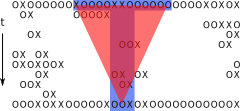
\includegraphics{overview}
    \end{center}
    \caption{
        An overview of the method for a neighbor-dependent model.
        The red triangle represents the ``range of influence'' of mutations on a site of interest (the site at the bottom corner of the triangle).
        The blue T shape is called a \emph{T-mer}, which is how our approximation to the process is parameterized.
        The bottom is called the \emph{base} of the T-mer, which is considered the outcome of a probabilistic process parameterized by additional \emph{overhang} sequence extending to the left and right of the base.%
        \label{fig:overview}
    }
\end{figure}

Before diving into a formal problem specification, we offer an intuitive explanation of how the method works.
The difficulty of context-sensitive models is that, in principle, one may have a sequence of events with cascading consequences that involves a lot of the sequence.
In the extreme case, one may have a sequence of mutations from, say, the left boundary of the sequence to the right boundary of the sequence, such that the probability of each mutation has been changed by that of the previous one.

However, the starting point of the work presented here is that for typical models such a sequence of events is improbable.
For that reason, we can perform computation using a local context which, although bigger than the context specified in the context-sensitive model, is much smaller than the entire sequence.
We call the building blocks of this computation \emph{T-mers} (Figure~\ref{fig:overview}) which parameterize transition probabilities for a small section of sequence (the \emph{base} of the T-mer) based on additional sequence (the \emph{overhang} of the T-mer).
We can bound the probability that the influence of a mutation outside the overhang of the T-mer will impact the sites at the base of the T-mer, which translates into an estimate of approximation error across the sequence when using a composite likelihood calculation based on T-mers.


%%%%%%% %%%%%%%%%%
\section{A general context-dependent model}

Consider a 1-dimensional grid of sites, each of which can take one of a finite set of states,
and that switch randomly between states according to a local set of rules.
We then observe a finite collection of these sites at only a few times,
Suppose that the dynamics are Markov:
writing $\calS$ for the set of possible states
and $X_i(t)$ for the state of site $i$ at time $t$,
we assume that $\{X(t)\}_{t \ge 0}$ is a Markov process on sequences of $L$ states $\calS^L$
for which the probability a given site changes state in a small amount of time
depends only on the sequence of states at nearby sites.

To formalize this notion of local dependence,
first define a \textit{pattern} to mean a contiguous sequence of states;
let $|u|$ denote the length of the pattern $u$.
Given $x \in \calS$,
let $x_i^{(h)} = (x_i, x_{i+1}, \ldots, x_{i+h-1})$ denote the pattern of $x$ of length $h$ beginning at location $i$.
% Recall we are focusing on finite sequences, and by default, we do not allow patterns to ``hang off'' the end of the sequence.
% This is natural in many situations, but in others we might want to other boundary conditions,
% modeling extant, but unobserved, neighbors.
% We will mention this when necessary.
The dynamics of our stochastic process are determined by the set of allowed transitions and associated rates:
given two patterns $u$ and $v$ of common length $h$,
saying ``pattern $u$ changes to $v$ at rate $\mu$'' means that
\[
    \P\{ X_i^{(h)}(t+dt) = v \given X_i^{(h)}(t) = u \} = \mu dt + o(dt),
\]
regardless of the location $i$ along the sequence.
If more than one pattern would match to cause the same change, their rates add.
Such a rule is defined by its ``transition triple'' $(\mu,u,v)$,
written as ``$u \to v$ at rate $\mu$''.
The set of all transition triples is denoted $\calT$.

\begin{example}[TASEP]
  The \emph{Totally Asymmetric Simple Exclusion Process} labels each site as ``empty'' or ``occupied'' (0 or 1, respectively),
  and says that each occupied site, independently at rate $\lambda$, checks the site to the right to see if it is empty,
  and if it is, moves there.
  This process therefore has only one transition triple:

  \begin{center}
    \begin{tabular}{c@{\quad$\to$\quad}c@{\quad at rate\quad }c}
      10  &   01   &  $\lambda$.
    \end{tabular}
  \end{center}

  \noindent
  This only has one parameter.
  If we allow particles to exit from the right, and new particles to enter from the left
  then from observing only starting and ending configurations
  we cannot tell with certainty which particles have moved where,
  so it is not obvious how to estimate the speed.
  However, summing over possible particle movements would allow us to
  compute the likelihood of a given configuration change,
  and so estimate the speed by maximum likelihood
  given an initial sequence, a final sequence and an elapsed time.

\end{example}


To allow more compact specification of models,
we also introduce a ``potential'':
suppose that there is a collection of patterns $\{p_i\}$
such that each occurrence of $p_i$ adds a quantity $e_i$ to the total ``energy'' of a sequence,
and that the rate at which each possible change occurs is modulated by a function of the energy difference the change would produce.
This is natural if that transition triples describe \emph{proposed} changes,
and that the probability a proposed change actually occurs depends on how much it affects the energy.

Concretely, let $\calP = \{(p_i, e_i)\}$ be a set of (pattern, energy difference) pairs,
and for any sequence $x$ define
$E(x) = \sum_i e_i\, n(x,p_i)$,
where $n(x,p_i)$ is the number of times the pattern $p_i$ occurs in $x$.
These will affect the rates through a nonnegative function $\phi$:
we declare that if the rate at which $x$ changes to $y$ as computed
from transition triples is $\mu$,
then the actual rate is
\[
    \mu \, \phi\left(E(y) - E(x)\right) .
\]
If $\phi(e)$ is not greater than 1, one way to think about this is that
the transition triples give ``proposed changes'',
but these changes only take effect with probability $\phi(E(y) - E(x))$.
We have described this idea in terms natural for a physics model such as an Ising model in which high energy configurations are disfavored, however it is also suitable for a population genetics model in which $\phi$ describes the probability of a mutant allele given a certain fitness change from the parent.

\begin{example}[Genomic GC content]
    A sequence of genome can be written using A, C, G, and T;
    in the most general model of independent mutation across sites, each of the 12 possible transitions occurs at its own rate.
    Furthermore, it is a well-known observation that in many species,
    adjacent, methylated CG dinucleotides (``CpG sites'') have a much higher mutation rate to TG and CA
    than either single nucleotide change under the independent model.
    Embellishing the single-nucleotide model with this additional rate results in the model defined by
    \begin{center}
      \begin{tabular}{c@{\quad$\to$\quad}c@{\quad at rate\quad }cc}
        $x$  &  $y$  &  $m_{xy}$ & for $x, y \in \{\nA,\nC,\nG,\nT\}$ and $x \neq y$ \\
        \nC\nG   &  \nT\nG   &  $\gamma$ & \\
        \nC\nG   &  \nC\nA   &  $\gamma$ &
      \end{tabular},
    \end{center}
    where $\gamma$ is the additional CpG rate above the base mutation rate.
    Note that for a given pair of sequences,
    a change $\nA\nC\nG \to \nA\nT\nG$ could have occurred by a $\nC \to \nT$ mutation
    via the independent-sites model,
    or by a $\nC\nG \to \nT\nG$ mutation;
    in such cases
    the total instantaneous rate at which ACG changes to ATG is the sum of the rates
    (in this example, $\gamma + m_{\nC\nT}$).
    % Although this means there are many possible parameterizations,
    % note that the model is identifiable, not overparameterized.

    Counteracting this trend towards increased G/C is GC-biased gene conversion \citep{glemin2015quantification},
    which is effectively a selective pressure against G or C bases.
    We model the evolution of a \emph{single} sequence, not a population of sequences,
    imagining this sequence to be the consensus sequence of the population.
    A new mutation with an effect $s$ on fitness that occurs
    in a population of effective size $N_e$ becomes ubiquitous, rather than dying out,
    with probability approximately $(1-\exp(-2 s))/(1-\exp(-2 s N_e))$ \citep{kimura1962probability}.
    If the mutation occurs at rate $\mu$ per individual, the total rate it occurs at in the population is $\mu N_e$.
    GC-biased gene conversion effectively means that sequences with more G/Cs are selected against.
    This is incorporated as follows: set the energy of pattern of pattern \nC{} or \nG{} to be $s$,
    so that $E(y)-E(x)$ is the net change in number of G's and C's multiplied by $s$.
    Also, assume a $\phi$ function expressed in terms of an energy difference $e$:
    \begin{align*}
        \phi(e) = (1-\exp(-2e))/(1-\exp(-2eN)).
    \end{align*}
    Thus, if a given change that occurs with rate $\mu$ would change a sequence $x$ to $y$,
    then $\mu \, N_e \phi(E(y)-E(x))$ is the rate at which the mutation
    appears and successfully takes over in the population.

\end{example}



\begin{example}[Gibbs sampling of the Ising model]
    In the Ising model, each site is labeled as either ``up'' or ``down'' ($+1$ or $-1$ respectively),
    imagined as a string of $n$ magnetic dipoles,
    and the energy associated with a given state $x$ is $E(x) = - \frac{1}{2} \beta \sum_{i=1}^{n-1} x_i x_{i+1} - \frac{1}{2} \gamma \sum_{i=1}^n x_i$.
    Here $\beta$ represents inverse temperature, and $\gamma$ represents the strength of the magnetic field (here scaled by temperature).
    The associated stationary distribution on configurations is proportional to $\exp(-E(x))$.
    The following process, also known as ``Glauber dynamics'', preserves the stationary distribution:
    each site, independently at rate $\lambda$,
    forgets its spin,
    and reconfigures to a state chosen with probability proportional to the stationary probability of the resulting configuration:
    Since $\exp(-E(x))/(\exp(-E(x))+\exp(-E(y))) = 1/(1+\exp(-(E(x)-E(y)))$,
    this is:
    \begin{center}
        \begin{tabular}{c@{\quad$\to$\quad}c@{\quad at rate\quad }c}
          $+$  &   $-$   &  $\lambda$ \\
          $-$  &   $+$   &  $\lambda$
        \end{tabular}
        \qquad and \qquad
        \begin{tabular}{cc}
        pattern  &  energy \\
        $+-$ or $-+$  &   $\beta$ \\
        $+$ &   $\gamma$
        \end{tabular}
    \end{center}
    and
    \begin{align*}
        \phi(e) = \frac{1}{1+\exp(-e)} .
    \end{align*}

    This process has been studied by XXX.
\end{example}


\paragraph{The generator matrix}
We now describe concretely how the set of transition rates on patterns determines the transition rate matrix for complete sequences, that is,
the $|\calS|^n \times |\calS|^n$ matrix $G(n)$ whose $(x,y)^\text{th}$ entry gives the instantaneous rate
with which the process in state $x \in \calS^n$ jumps to state $y \in \calS^n$.
Recall that $x_i^{(h)} = (x_i, x_{i+1}, \ldots, x_{i+h-1})$ denotes the subsequence of length $h$ beginning at location $i$.
For each $1\le i \le n$, pattern length $h > 0$, and patterns $u,v \in \calS^h$ define the relation
\[
x \xrightarrow{i,u,v} y \qquad \text{iff} \qquad \begin{cases}
  x_k = y_k \quad &\text{for } k<i \\
  x_{i+k} = u_k \quad &\text{for } 0 \le k < h \\
  y_{i+k} = v_k \quad &\text{for } 0 \le k < h,\ \text{and} \\
  x_k = y_k \quad &\text{for } k\ge i+h ,
\end{cases}
\]
i.e., if $x$ and $y$ match except at positions $i,i+1,\ldots,i+h-1$,
and for those positions $x$ matches with $u$ while $y$ matches with $v$.
Let $\calT$ be the set of these transition triples.

As noted above, there may be more than one way to mutate a sequence $x$ to get $y$:
for each position $i$, let $J(i,x,y)$ be those transitions in $\calT$ that can be applied at $i$
to change $x$ into $y$, i.e.,
\[
    J(i,x,y) = \{ (\mu,u,v) \in \calT \st x \xrightarrow{i,u,v} y \}.
\]
The rate ${G(n)}_{x,y}$ is then the sum of all matching transition rates,
multiplied by the fitness term,
namely
\begin{align} \label{eqn:G_defn}
    {G(n)}_{x,y} = \phi\left(E(y)-E(x)\right) \, \sum_{i=1}^n \sum_{(\mu, u, v) \in J(i,x,y)}  \mu ,
\end{align}
and if there are no triples $(\mu,u,v)$ with $x \xrightarrow{i,u,v} y$ for some $i$, then ${G(n)}_{x,y}=0$.
Indeed, we anticipate this matrix to be sparse because for most pairs $(x,y)$ there are no transition triples that can modify $x$ to make $y$.

In principle, this gives us the transition probabilities for the process by a matrix exponential:
\begin{align} \label{eqn:full_likelihood}
    p_n(t;x,y) := \P\{ X(t) = y \mid X(0) = x \} = {\left(e^{tG(n)}\right)}_{xy} ,
\end{align}
which would then provide a route to parameter estimation.
In practice, the size of these matrices makes direct application obviously impractical for anything but very small $n$.
This paper proposes an alternate strategy.


\section{Simulation}

First, it will be useful for later proofs to have an explicit construction of the process,
also used for simulation,
using a variant of the ``jump chain representation'', also known as the ``Gillespie algorithm''
or ``uniformization'' \citep{hobolth2009simulation}.
Briefly, this  works by first sampling a homogeneous Poisson process of times and locations of possible changes,
at an appropriate rate $\mu^*$ per site,
and then resolving each possible change in temporal order.
(Note that these ``possible changes'' are different than the ``proposed changes'' described above
in terms of the energy model.)
The rate $\mu^*$ should be the maximum ``local'' rate at which transitions occur, across sites and transition outcome states:
\[
    \mu^* = \max \left\{ \sum_{y \in \calS^L} \sum_{(\mu, u, v) \in J(i,x,y)} \mu \qquad \st x \in \calS^L, \quad 1 \le i \le L \right\} .
\]
Now sample possible changes:
in a sequence of length $L$, over a time period $t$,
first draw the number of possible changes, $N$,
from a Poisson distribution with mean $\mu^* t L$,
and then choose the times $s_k$ and locations $i_k$
at which possible changes occur uniformly
over $[0, t]$ and $\{1, 2, \ldots, L\}$ respectively.
Order the possible change times, so that
\[
    0 < s_1 < \cdots < s_N < t .
\]
(Note that this is equivalent to saying that possible
changes occur at rate $\mu^*$ independently at each of the $L$ sites.)
Now, suppose we have determined the state just before time $s_k$ to be $X(s_k) = x$.
Then, a new state is then chosen at position $i_k$
with probability proportional to the corresponding rate, i.e.,
out of the possible transitions $\calT$, the $j^\text{th}$ one is chosen
with probability
\[
q_j = \begin{cases}
    % TODO peter, fix notation, please.
    \mu^{(j)}/\mu^* \qquad & \text{if } x_i^{(|u^{(j)}|)} = u^{(j)}  \\
    0 \qquad & \text{otherwise.}
\end{cases}
\]
The remaining probability $q_0 = 1-\sum_{j=1}^{|\calT|} q_j$
gives the probability that the state remains the same.
(By construction of $\mu_*$, $q_0\ge 0$.)
If triple $(\mu^{(j)}, u^{(j)}, v^{(j)})$ is chosen, then
the substring of $x$ matching $u^{(j)}$ that begins at position $i$
is replaced with $v^j$ to produce $X(s_k)$.

For instance, to simulate the TASEP, one has only to let $\mu^*=\lambda$, and at each $c_{ij}$
check if at site $i$ there is a 1 followed by a 0,
and if so, switch them.


\section{Inference}

\peter{refer to figure}

The problem at hand is to infer the parameters of the model based on the final state of the model after it has evolved from some known initial state.
% If the sequence is long enough and not too much time has gone by
% this should be feasible -- there should be enough information in our observations to do this reliably.
% If the time is too large, the process may ``saturate'' --
% if there are many changes at most sites, then in at least most models,
% we will lose most information about the dynamics,
% retaining information only about the parameters that affect the stationary distribution.
% In TASEP with any boundary conditions, we lose all information as it approaches stationarity,
% while in the Ising model we have information about the temperature $\beta$ and magnetic field $\gamma$ but not the speed of changes, $\lambda$.
% In the CpG model it is not immediately clear what information is retained.
How can we extract the information?
These are Markov processes, on the state space $\calS^n$,
so the full likelihood function is given by \eqref{eqn:full_likelihood},
but doing anything with the $|\calS|^n \times |\calS|^n$ matrix $G_n$ is clearly infeasible even for moderately sized $n$.
We can, however, compute \eqref{eqn:full_likelihood} for smaller $n$,
so the first thing that one might think to do is to break the sequence up into many blocks of length $m$,
and treat these as independent.
Then, defining $p_m(t;x,y)$ to be the probability that a string $x$ of length $m$ evolves to string $y$ over time $t$,
we would obtain the approximate likelihood function
\[
  \prod_{k=0}^{n/m} p_m(x_{km+1}^{(m)},y_{km+1}^{(m)}) .
\]
However, this ignores dependencies between neighboring blocks,
so it is not clear how good this approximation might be.
% Intuitively, we want to increase the size of the context
% -- and the likelihood thus obtained is asymptotically correct for $m$ large,
% but computationally, we are stuck with small values of $m$.

\begin{figure}
    \begin{center}
        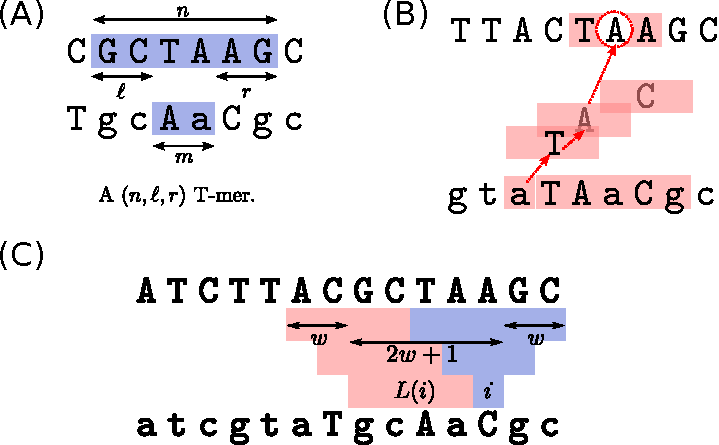
\includegraphics{Tmer-dependency}
    \end{center}
    \caption{
        \textbf{(A)} A $(6,2,2)$ T-mer.
        Nonmutated sites are shown in lower case letters.
        The ``base'' of the T-mer is the lower central
        string of length $m = n - \ell - r$.
        \textbf{(B)}
        The three mutations have extended the influence of the circled \nA{}
        in the initial sequence (top)
        to the six positions colored red in the final sequence.
        The rate of each mutation depends on its' neighboring sites,
        i.e., with a window of width $w=1$.
        Red dotted arrows show the propagation of dependency
        between the circled \nA{}
        and the third site in the final sequence (bottom).
        \label{fig:Tmers}
    }
\end{figure}



The key insight we use is that by including neighboring sequence context in the \emph{initial} sequence only,
we can compute \emph{something} correctly,
and that something will be sufficient to compute the full likelihood
to an arbitrarily good approximation.
%EM do we really want x and y here, which I've been thinking of as being the full sequence?
%EM Note we'll need to change a and b below.
To do this, let $p_{n,\ell,r}(x,y)$ for $\ell + r < n$ denote
the probability that an initial subsequence $x$ of length $n$, after time $t$,
is found to match a smaller subsequence $y$ of length $n-\ell-r$, offset by $\ell$ sites.
This central, smaller subsequence is called the ``base'' of the T-mer.
We refer to such patterns as \emph{T-mers}, as depicted in Figure~\ref{fig:Tmers}.
We emphasize that the overhang of the T-mers is typically bigger than the
context-sensitivity width of the underlying model (Figure~\ref{fig:overview}).

These $p_{n,\ell,r}(x,y)$ probabilities can be found by marginalizing $p_m$,
summing over the possible inital and final substrings of $x$
(denoted $a$ and $b$):
\begin{align}
    p_{n,\ell,r}(t;x,y)
    &=
    \sum_{a \in \calS^\ell} \sum_{b \in \calS^r} p_n(t;x,a \join y \join b) ,
    \quad
    \text{for}\; x \in \calS^n, \; y \in \calS^{n-\ell-r} ,
    \label{eq:pmMarg}
\end{align}
where $a \join y \join b$ is the sequence composed of concatenating $a$, $y$, and $b$ together in that order.
We expect $p_{n,\ell,r}(x,y)$ to be asymptotically correct when $\ell$ and $r$ are large (and $t$ is fixed).
In Appendix~\ref{ss:approx_pf}, we show that this is so, namely that
the probability a given subsequence of length $n$ matching $x$
is later observed to have its center matching $y$
is close to $p_{n,\ell,r}(x,y)$, regardless of wider context.
Formally, for each $i$,
\begin{align} \label{eqn:window_approx}
    \P\{ X_{i+\ell}^{(n-\ell-r)}(t) = y \mid X_i^{(n)}(0) = x \}
    \approx
    p_{n,\ell,r}(x,y)
    .
\end{align}


%%%%%%
\subsection{Full likelihood}

What we actually want is the \emph{full likelihood} $\like(y|x)$,
the probability that a given sequence $x$ evolves into another, $y$, over a given period of time.
This can be computed as the product of the probability of each site in $y$
given $x$ and all sites in $y$ further to the left.
Defining $x_{<i}=(x_1, \ldots, x_{i-1})$ to be the subsequence to the left of $i$, this is:
\begin{align*}
    \like(y \mid x) &= \prod_i \P\{ Y_i = y_i \given Y_{<i} = y_{<i} \ \text{and}\; X=x \} .
\end{align*}
It turns out that
we can approximate the terms in this sum
by discarding approximately independent sites from the conditioning.
These approximately independent sites are exactly those that are too far away from a given site to impact its evolution.
Recall that the last base of $x_i^{(h)}$ is $x_{i+h-1}$.
So, $x_{i-3\ell}^{(4\ell+1)}$ runs from $i-3\ell$ to $i + \ell$, inclusive, while $y_{i-2\ell}^{(2\ell+1)}$ runs from $i-2\ell$ to $i$, inclusive.
If $\ell$ is long enough that approximation~\eqref{eqn:window_approx} holds, then:
\begin{align} \label{eqn:full_approx}
    \begin{split}
    \P\{ Y_i = y_i \given Y_{<i} \ \text{and}\; X=x \}
    &\approx
        \P\{ Y_i = y_i \given Y_{i-2\ell}^{(2\ell+1)} \;\text{and}\; X_{i-3\ell}^{(4\ell+1)} \}  \\
    &=
        \frac{
            p_{2\ell+1,\ell,\ell}(x_{i-3\ell}^{(4\ell+1)}, y_{i-2\ell}^{(2\ell+1)})
        }{
            p_{2\ell+1,\ell,\ell+1}(x_{i-3\ell}^{(4\ell+1)}, y_{i-2\ell}^{(2\ell)})
        }.
    \end{split}
\end{align}

%EM I think you said that we could just treat the state of all positions before the beginning of the sequence and after the end as having another distinct state. If that's true I can write it out.

Let $A_{n, \ell, r}(x,y)$ be the product of all probability of all $(n, \ell, r)$ T-mers transitioning from $x$ to $y$, i.e.\
\[
A_{n, \ell, r}(x,y) = \prod_{i=1}^L p_{n, \ell, r}\left(x_{i-\ell-m}^{(n)}, y_{i-m}^{(n-\ell-r)}\right).
\]

We can then express our likelihood as

\[
    \like(y \mid x) = \frac{ A_{2\ell+1, \ell, \ell}(x,y) }{ A_{2\ell+1, \ell, \ell+1}(x,y) }.
\]

% Define $n_\ell(x,y;a,b)$ to be the number of times pattern $a$ is seen in sequence $x$
% matched to pattern $b$ in $y$ at a position offset by $\ell$.
% Then
% \begin{align}
%     \log \like(y|x)
%     &\approx
%         \sum_{a \in \calS^n} \sum_{b \in \calS^{n-2\ell}} n_\ell(x,y;a,b) \log p_{n,\ell,\ell}(a,b)
%         -
%         \sum_{c \in \calS^n} \sum_{d \in \calS^{n-2\ell-1}} n_\ell(x,y;c,d) \log p_{n,\ell,\ell+1}(c,d)
% \end{align}
See Appendix~\ref{ss:approx_pf} for a more rigorous statement and proof,
and the next section for some intuition.

%%%%%
\subsection{Choice of overhang}

The approximations in~\eqref{eqn:window_approx} and~\eqref{eqn:full_approx} hold
if the overhang, $\ell$, is long enough.
We present intuition about these formulas here, which provides a way to pick the overhang lengths $\ell$ and $r$;
a precise statement is given in Appendix~\ref{ss:approx_pf}.
Suppose that each instantaneous change depends on positions at most $w$ sites away,
and refer to $w$ as the ``window width''.
Then, the mutation process at any particular site
depends on the initial sequence at that site and within distance $w$ on either side\ldots
\emph{and} the outcomes of any mutations that have occurred within that window.

Therefore, the sequence at a particular site may directly affect the process at the neighboring $w$ sites on either side.
If another change happens, say, at the end of this window,
then the indirect effects of this change may extend out to $2w$ sites.
In this way, the influence of the sequence at each site extends outwards, as shown in Figure~\ref{fig:Tmers} --
so if we take the overhangs long enough that this dependency is unlikely to extend to the base of the T-mer,
the approximation will be good.
As we show in Section \ref{ss:approx_pf}, if the overhangs are $\ell = r = kw$,
then the error in approximation \eqref{eqn:window_approx}
is bounded by the probability that there are more than $k$ changes in a given window of length $w$.
Concretely, sites further away than $kw$ only matter if there is a chain of at least $k$ intervening mutations
-- which is unlikely if $k$ is much larger than the expected number.

For instance, in the CpG model the window width is $w=1$
because the process only depends on neighboring sites;
and if the sequence has evolved for time $t$ then we expect no more than a Poisson($\lambda t$) number of changes at each site.
If $\lambda t = 0.75$ (three-quarters of the sequence will have changed!),
then taking $\ell = r = 3$ allows us to compute Tmer probabilities to within an error of 0.007,
since this is the probability that a Poisson with mean 0.75 will be larger than 3.
If $\lambda t = 0.25$ we would do even better with $\ell = r = 2$.

To obtain the full likelihood, in \eqref{eqn:full_approx}, in addition to an overhang of $\ell$
we needed the base of the T-mer to be of length $2\ell+1$.
This is because we have also conditioned on the final sequence to the left of the focal site, $Y_{<i}$,
and although the process at $i$ only depends on events within $\pm \ell$,
these events may affect other sites in $Y$ going back a distance $2\ell$.


%%%%%%%%
\subsection{Model fit and model selection}

Fitting a model to nucleotide data would likely require iterative modification of the model.
The difference between observed and expected T-mer counts provide a good assessment of how and whether a model can be improved.
These \emph{residual} counts are usually most usefully computed for T-mers shorter than those used to fit the model.
For each T-mer $(a,b)$, write $O_{a,b}$ for the number of this T-mer observed in the data,
and $E_{a,b}$ for the number expected under the model.
(The expected number is the number of occurrences of $a$ in the initial sequence
multiplied by the probability $p_{n,\ell,r}(t;a,b)$, where $n$ is the length of $a$,
and $\ell$, $r$ are the appropriate overhangs.)
If the T-mers were nonoverlapping, this would form a standard contingency table,
and standard practice would be to divide the residuals by the square root of the expected counts
and compare these to a standard Normal distribution.
However, there are are $n$ possible such tables --
so, we compute normalized residuals as
\begin{align}
    Z_{a,b} = \frac{ O_{a,b} - E_{a,b} }{ \sqrt{n E_{a,b}} },
\end{align}
which is equivalent to averaging the $z$-scores of the $n$ possible tables of nonoverlapping counts.
These can then be compared to a standard Normal distribution.

%EM This is stepwise model addition.

%%%%%%%%%%%
\section{Computation}

For inference, we need to compute the $|\calS|^{n} \times |\calS|^m$ matrix $F$ whose $(a,b)^\text{th}$ entry is $p_{n,\ell,r}(t,a,b)$,
for various $t$.
This matrix is a projection of the $|\calS|^{n} \times |\calS|^{n}$ matrix whose $(a,c)^\text{th}$ entry is
\begin{align}
    p_{n}(a,c) = \left( e^{t G(n)} \right)_{a,c} ,
\end{align}
where $G(n)$ is the sparse $|\calS|^{n} \times |\calS|^{n}$ matrix defined in \eqref{eqn:G_defn}.
The ``projection'' we need just marginalizes over long (i.e.\ length $n$) patterns $c$ that match the shorter (i.e.\ length $m$) pattern $b$
as in \eqref{eq:pmMarg}:
if we define the $n \times m$ matrix $U$ so that $U_{cb}=1$ if $c_\ell^m=b$ and $U_{cb}=0$ otherwise,
then
\begin{align} \label{eqn:Tmer_trans}
    p_{m,\ell}(t,a,b) = \sum_{c \in \calS^{n}} \left( e^{t G(n)} \right)_{ac} U_{cb} ,
\end{align}
so in fact we don't need the entire matrix $e^{t G(n)}$,
just the product of this matrix with each of the columns of $U$.
Modern techniques in sparse matrix computation (e.g., Krylov methods) provide efficient ways to do this.

Using the R package expm \citep{R_expm}, this makes computation quite feasible:
with four possible states and $\ell=2$ and $m=1$, so that $G(n)$ is a $1024 \times 1024$ matrix,
computing $e^{t G(5) }$ takes 13 seconds, while computing $e^{t G(5)} U$ takes only 0.3 seconds.
%EM In the above, don't we only provide the recipe for the full likelihood when m = 2 ell + 1?
Increasing to $\ell=4$ and $m=1$ or $\ell=3$ and $m=2$ is still feasible, taking $e^{t G(8)} U$ in 42 and 47 seconds, respectively
(and much longer for the whole matrix $e^{t G(8)}$).

Although we haven't used such tools here, taking the derivative with respect to $t$ can also be performed using sparse matrix operations.


\paragraph{Sparsity and updating $G$}
We can also take advantage of the sparsity of $G$ to perform efficient computation of the likelihood
under many sets of parameters.
Let's assume that the T-mers only allow single-position changes.
First note that in this case $G(n)$ has
$(1+m(|\calS|-1)) |\calS|^{n}$ nonzero entries, since each of the $|\calS|^{n}$ can change in $m$ places.
This will determine how the computation scales with $m$, $n$, and $|\calS|$,
once we precompute a number of things.
Let $g = (g_1, \ldots, g_d)$ be the nonzero entries of $G$, in some fixed ordering;
sparse matrix representations of $G$ store only $g$ along with information about the rows and columns these are found in.
%EM Here we are using lower j, rather than our "new" notation setup, but it doesn't seem like a big deal. This is a local note.
Each $g_i$ is a linear combination of mutation rates $\mu_j$,
multiplied by a function ($\phi$) of a linear combination of energy coefficents $e_j$,
say $g_i = \sum_j A_{ij} \mu_j \phi(\sum_k B_{ik} e_k)$,
so by precomputing the matrices $A$ and $B$ we can update $G$ with new parameter values
using only two matrix multiplications and evaluation of $\phi()$ over a vector.
This remains efficient to perform in interpreted languages such as R,
since each step is carried out by lower-level compiled code (e.g., optimized linear algebra libraries).
% This is true if the boundary conditions are circular, mean-value, or neither.

%%%%%%%%
\section{Phylogenetic inference}

In phylogenetic applications, rather than ``before'' and ``after'' observations,
%EM Describe the root sequence, or a prob distribution on it?
%EM We want to be able to talk about the probability of seeing a certain n-mer... is that obvious what that random process is on the whole-sequence level?
we get two (or more) observations evolved from a common root.
In the simplest case of two tips we have two processes $X$ and $Y$,
with identical starting states $X(0)=Y(0)$,
observed only at times $t_X$ and $t_Y$ respectively.

If the approximation described above holds,
then we can write the probability that we see (long) pattern $x$ in $X(t_X)$ juxtaposed with (short) pattern $y$ in $Y(t_Y)$
using the pattern frequencies at the root.
%EM Could we make it \rho_I to emphasize that it's a random quantity?
Concretely: pick a random location $I$ in the sequence and let $X_{I-\ell}^{n}(0) = \rho$ be the (long) pattern seen there at the root.
Write $\pi(z)$ for the frequency of a given pattern $z$ in $X(0)$, i.e., $\P\{\rho=z\}=\pi(z)$.
% Given the corresponding pattern in $X(t_X)$, the distribution of $\rho$ is proportional to
% \[
%     \P\{ \rho=z \mid X_{I-\ell}^{n}(t_X)=x\} \propto \pi(z) p_{n}(t,z,x) .
% \]
The probability that we see $x$ and $y$ at the random location $I$ is
\begin{align} \label{eqn:phylo_likelihood}
    \P\{X_{I-\ell}^{n}(t_X)=x \text{ and } Y_I^\ell(t_Y)=y \} = \sum_{z \in \calS^{n}} \pi(z) \, p_{n,\ell,r}(t_X,z,x) \, p_{n,\ell,r}(t_Y,z,y) .
\end{align}
This can be computed without much more effort than the simpler case above,
given the frequencies at the root, as described in greater generality below.
These calculations can be done using the same sparse matrix methods as above.
For instance, to compute
\[
    %EM This is super clever!
    \sum_{z \in \calS^{n}} \pi(z) \, p_{n,\ell,r}(t_X,z,x) \, p_{n,\ell,r}(t_Y,z,y)
    = \sum_{z \in \calS^{n}} \left( e^{t_X G(n)} \right)_{zx} \pi(z) \sum_{w \in \calS^{n}} \left( e^{t_Y G(n)} \right)_{zw} U_{wy} ,
\]
we can first compute $\sum_w \left( e^{t_Y G(n)} \right)_{zw} U_{wy}$ as above,
multiply rows by $\pi(z)$, and then matrix multiply by the transpose of $e^{t_X G(n)}$.


%EM It seems like we'd like to write out how this works for the entire set of sequences, as you did for the "full likelihood" section.
%EM I think we have a bunch of ratios as before, where r is extended by 1 in the numerator?


%EM I think this should be pruning, not peeling.
%EM Want to check the modifications made above before continuing those to here.
\subsection{Phylogenetic peeling}

The general case is a modification of Felsenstein's ``peeling'' algorithm.

\begin{figure}
    \begin{center}
    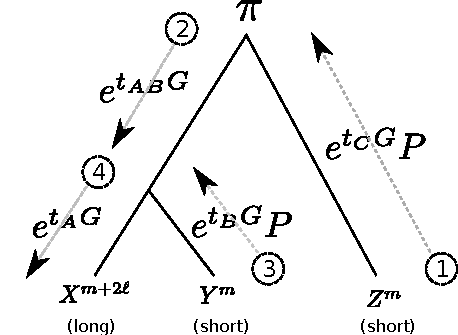
\includegraphics{peeling-schematic}
    \end{center}
    \caption{
        A depiction of the four steps in computing the likelihood of finding particular ``short'' subsequence at $Y$ and $Z$
        given the ``long'' subsequence at $X$: see text for details.
        \label{fig:peeling}
    }
\end{figure}

To compute the likelihood on a more complicated tree, consider the following,
with the three-taxon tree of figure \ref{fig:peeling} as an example,
where we are counting occurrences of (long) $n$-tuples in taxon $X$,
and (shorter) $m$-tuples in taxa $Y$ and $Z$.
The likelihood in this example is found by summing over the root state (the summation over $u$)
and the interior node ($v$):
\begin{align} \label{eqn:three_taxa_likelihood}
  \begin{split}
    & \P\{X_{I-\ell}^{n}=x \text{ and } Y_I^\ell=y \text{ and } Z_I^\ell=z \} \\
    &\qquad = \sum_{u \in \calS^{n}} \pi(u) p_{m,\ell}(t_C,u,z) \sum_{v \in \calS^{n}} p_{n}(t_{AB},u,v) p_{n}(t_{A},v,x) p_{m,\ell}(t_B,v,y)
  \end{split}
\end{align}
The steps for computing this are then:
\begin{enumerate}

  \item Compute $M_1(u,z) = p_{m,\ell}(t_C,u,z)$ (a $|\calS|^{n} \times |\calS|^m$ matrix)

  \item Compute $M_2(v,z) = \sum_{u \in \calS^{n}}  p_{n}(t_{AB},u,v) \pi(u) M_1(u,z)$ (still a $|\calS|^{n} \times |\calS|^m$ matrix)

  \item Compute $M_3(v,y) = p_{m,\ell}(t_B,v,y)$ (a $|\calS|^{n} \times |\calS|^m$ matrix)

  \item Compute $M_4(x,(y,z)) = \sum_{v \in \calS^{n}} p_{n}(t_{A},v,x) M_2(v,z) M_3(v,y)$ (stored as a $|\calS|^{n} \times |\calS|^{2m}$ matrix).

\end{enumerate}
Then $M_4$ gives all the likelihoods.
This is depicted in the figure, writing $\left(e^{tG}\right)_{ab}$ for the matrix $p_{n}(t,a,b)$,
and $P$ for the projection matrix that gives $p_{m,\ell}(t,a,b) = \left( e^{tG} P\right)_{ab}$.


In total there are $|\calS|^{3m+2\ell}$ possible data combinations.
However, we can reduce dimensionality by replacing the last step with
\begin{enumerate}

  \item[4'.] Compute $M_4(x,w) = \sum_{v \in \calS^{n}} p_{n}(t_{A},v,x) M_3(v,w) M_4(v,w)$ (stored as a $|\calS|^{n} \times |\calS|^{m}$ matrix).

\end{enumerate}
i.e., only computing the likelihood for cases with $y=z=w$.
On a three-taxon tree it is not clear that this is desirable, since missing out on double transitions
might be a significant loss of information,
but on larger trees it seems likely that we'd want to restrict to combinations with most sites agreeing across the tree.
(Note, however, that one should not first look at the data, observe which combinations $(y,z)$ were most common, and then restrict to only those!)

The algorithm for a general tree is written out in Appendix \ref{ss:peeling_algorithm}.


%%%%%%%%%%%
\subsection{Hominid data}

We also applied the model to human--chimpanzee divergence data,
restricting the comparison to putative regulatory sequences,
avoiding the additional constraints of coding sequences.
To do this, we extracted regions in the human (hg38)--chimpanzee (panTro4) alignment % \citep[from the UCSC Genome Browser][]{pantroalign}
according to four types of regulatory feature in the Ensembl Regulatory Build \citep[release 81][]{zerbino2015ensembl}:
``CTCF binding site'', ``enhancer'', ``open chromatin region'', and ``promoter flanking region''.
These were furthermore divided into regions that either did or did not overlap a transcription start or end site of a known gene
from the hg38 Annotations Database \citep{kent2002human}
and filtered for length:
aligned regions below either 3000bp (promoter flanking regions) or 1000bp (all other types).
We then counted Tmers of appropriate length in each of the eight resulting sets of aligned regions, omitting any Tmers that included gaps or repeat-masked positions,
and fit models separately to each of the eight data sets.

We constructed models from three, nested, sets of mutation motifs.
All models are strand-symmetric.
\begin{itemize}
    \item[(basic)]
        Single-base changes, with separate rates for transitions ($\mu_v$),
        \nA$\leftrightarrow$\nT{} ($\mu_{AT}$), \nC$\leftrightarrow$\nG{} ($\mu_{CG}$),
        and other transversions ($\mu_{r}$):
          \begin{center}
            \begin{tabular}{c@{\quad$\to$\quad}c@{\quad at rate\quad }c|c@{\quad$\to$\quad}c@{\quad at rate\quad }c|c@{\quad$\to$\quad}c@{\quad at rate\quad }c}
                \nT  &   \nA   &  $\mu_{AT}$ & \nA  &   \nG   &  $\mu_{r}$ & \nA  &   \nG   &  $\mu_{v}$ \\
                \nA  &   \nT   &  $\mu_{AT}$ & \nG  &   \nA   &  $\mu_{r}$ & \nG  &   \nA   &  $\mu_{v}$ \\
                \nC  &   \nG   &  $\mu_{CG}$ & \nC  &   \nT   &  $\mu_{r}$ & \nT  &   \nC   &  $\mu_{v}$ \\
                \nG  &   \nC   &  $\mu_{CG}$ & \nT  &   \nC   &  $\mu_{r}$ & \nC  &   \nT   &  $\mu_{v}$ \\
            \end{tabular}
          \end{center}

      \item[(CpG)] In addition to the above, an additional CpG rate:
          \begin{center}
            \begin{tabular}{c@{\quad$\to$\quad}c@{\quad at rate\quad }c}
                CG  &   TG   &  $\nu_{CpG}$ \\
                CG  &   CA   &  $\nu_{CpG}$ \\
            \end{tabular}
          \end{center}

      \item[(repair)] In addition to the above, we included a collection of mutation motifs associated with known DNA lesion/repair pathways
          curated from the literature \citep[reviewed in][]{sale2012yfamily,goodman2013translesion,roberts2014hypermutation,cobey2015evolution,goodman2002errorprone}:
          deamination due to repair of UV-induced pyramidine dimers \citep[$\mu_{UV}$,][]{sale2012yfamily,sinha2002uvinduced};
          repair of guanine adducts at CpG sites \citet[$\mu_g$,][]{pfeifer2006mutagenesis};
          deamination by AID \citep[$\mu_{AID}$,][]{teng2007immunoglobulin,kasar2015wholegenome};
          deamination by members of the APOBEC family \citep[$\mu_\APOBEC$,][]{alexandrov2013deciphering};
          and repair by error-prone polymerases pol $\eta$ \citep[$\mu_\eta$,][]{alexandrov2013deciphering};
          and pol $\iota$ \citep[$\mu_{\iota}$,][]{roberts2014hypermutation,maul2016polymerase}.
          These are denoted here using ambiguity codes
          \nR{}: \nA{} or \nG{},
          \nY{}: \nC{} or \nT{},
          \nW{}: \nA{} or \nT{}, and
          \nS{}: \nC{} or \nG{};
          so for instance
          ``\nT\nC\nW$\to$\nT\nT\nW''
          means that both
          \nT\nC\nA$\to$\nT\nT\nA{}
          and
          \nT\nC\nT$\to$\nT\nT\nT{}
          share the same mutation rate.
          \noindent
      \begin{center}
          \begin{tabular}{c@{\;\;$\to$\;\;}c@{\;\; {\small at rate}\;\; }c|c@{\;\;$\to$\;\;}c@{\;\; {\small at rate}\;\; }c}
            \nC\nG     &   \nC\nT      &  $\mu_{g}$      & \nA\nA       &   \nA\nG       &  $\mu_{\iota1}$   \\
            \nC\nG     &   \nA\nG      &  $\mu_{g}$      & \nT\nT       &   \nC\nT       &  $\mu_{\iota1}$   \\
            \nT\nC     &   \nT\nT      &  $\mu_{UV}$     & \nA\nA       &   \nG\nT       &  $\mu_{\iota2}$   \\
            \nG\nA     &   \nA\nA      &  $\mu_{UV}$     & \nT\nT       &   \nA\nC       &  $\mu_{\iota2}$   \\
            \nC\nC     &   \nC\nT      &  $\mu_{UV}$     & \nT\nC\nW    &   \nT\nT\nW    &  $\mu_{\APOBEC}$  \\
            \nG\nG     &   \nA\nG      &  $\mu_{UV}$     & \nT\nC\nW    &   \nT\nG\nW    &  $\mu_{\APOBEC}$  \\
            \nC\nC     &   \nT\nT      &  $\mu_{UVd}$    & \nS\nG\nA    &   \nS\nA\nA    &  $\mu_{\APOBEC}$  \\
            \nG\nG     &   \nA\nA      &  $\mu_{UVd}$    & \nS\nG\nA    &   \nS\nC\nA    &  $\mu_{\APOBEC}$  \\
            \nT\nA     &   \nT\nG      &  $\mu_{\eta}$   & \nW\nR\nC\nY &  \nW\nR\nT\nY  &  $\mu_{\AID}$     \\
            \nT\nA     &   \nC\nA      &  $\mu_{\eta}$   & \nR\nG\nY\nS &  \nR\nA\nY\nS  &  $\mu_{\AID}$
        \end{tabular}
      \end{center}

\end{itemize}

The mutational motifs included above are far from complete
-- context-specific affinities and error rates \textit{in vivo}
are not known for most DNA repair pathways --
but neither do they exhaust the hypotheses available in the literature.
For instance, many enzymes act more than once locally when they act,
such as AID \citep{senavirathne2015activationinduced} or error-prone polymerases involved in repair \citep{maul2016polymerase}.


%%%%%%%
\section{Results}

%%%%%%%%%%%
\subsection{Stepwise model selection}

In exploratory application to real data, how does one decide when to stop adading mutational motifs?
Perhaps the simplest method conceptually is to
(a) fit a simple model,
(b) choose new motifs to add based on statistically significant residuals,
(c) repeat until no residuals are statisically significant.
To test this method,
we simulated a single sequence of $10^6$ nucleotides
for one unit of time
under the model given in Table \ref{tab:cpg_results},
obtained by embellishing the basic CpG hypermutability
with the longer mutational motif identified by \citet{harris2015evidence}.
%     \begin{center}
%       \begin{tabular}{c@{\quad$\to$\quad}c@{\quad at rate\quad }cc}
%         $x$  &    $y$  &  $m_{xy}$ & when $x \neq y \in \{\nA,\nC,\nG,\nT\}$  \\
%         \nC\nG     &  \nT\nG     &  $0.4$ & \\
%         \nC\nG     &  \nC\nA     &  $0.4$ & \\
%         \nT\nC\nC  &  \nT\nT\nC  &  $0.1$ & \\
%         \nA\nG\nG  &  \nA\nA\nG  &  $0.1$ &
%       \end{tabular} ,
%     \end{center}
% with $m_{AT}=m_{TA}=0.1$, $m_{CG}=m_{GC}=0.15$, $m_{AC}=m_{TG}=m_{AG}=m_{TC}=0.08$, and $m_{CA}=m_{GT}=m_{CT}=m_{GA}=0.12$.
% Note the model is symmetric under reverse complementation.
The resulting sequences differed at 28.5\% of the sites.
We then fit an unconstrained model of single-nucleotide substitution using (5,1,1) T-mers
(three sites at the base with an overhang of one on each side)
using a constrained quasi-Newton method (``optim(.., method='L-BFGS-B')'' in R).
The top and bottom of the table of (2,1,0) and (2,0,1) T-mer residuals of this model were as follows:
% cpg-plus-epsilon/32140/base-model-fit-5-3-l1-resids.2.1.l0.tsv
% cpg-plus-epsilon/32140/base-model-fit-5-3-l1-resids.2.1.l1.tsv
    \begin{center}
        \begin{tabular}{ccrrrr}
                $x$ & $y$ & observed &   expected &    residual &  $Z$ \\
                \hline
                \nC\nG  & \nC\_   & 100410   &  120303    & -19892.50   &	-40.55  \\
                \nC\nA  & \nT\_   &  19884   &   28350    &  -8466.43   &	-35.55  \\
                \nC\nT  & \nT\_   &  19998   &   28061    &  -8063.46   &	-34.03  \\
                \nC\nC  & \nT\_   &  23673   &   28177    &  -4503.96   &	-18.97  \\
                \nG\nG  & \nC\_   &  17742   &   19418    &  -1675.92   &	 -8.50  \\
                \nC\nG  & \nG\_   &  18450   &   19478    &  -1028.34   &	 -5.21  \\
                \nA\nG  & \nC\_   &  10968   &   11760    &   -791.73   &	 -5.16  \\
                \nG\nG  & \nG\_   & 118805   &  120975    &  -2170.25   &    \\
                \hline
                \nA\nG  & \nT\_   &  17280   &   16515    &    765.20   &  4.21   \\
                \nG\nT  & \nC\_   &  20490   &   19507    &    983.44   &  4.97   \\
                \nG\nG  & \nT\_   &  20929   &   19278    &   1650.83   &  8.40   \\
                \nC\nC  & \nC\_   & 124149   &  119880    &   4268.52   &  8.71   \\
                \nG\nG  & \nA\_   &  30483   &   28288    &   2195.34   &  9.22   \\
                \nC\nT  & \nC\_   & 126957   &  119389    &   7567.92   & 15.48   \\
                \nC\nA  & \nC\_   & 128673   &  120619    &   8054.46   & 16.39   \\
                \nC\nG  & \nT\_   &  49311   &   28276    &  21034.85   & 88.45   \\
                \hline
                \hline
                \nC\nG  &  \_\nG  &  100803  &  120541  &  -19737.80  &  -40.19 \\
                \nT\nG  &  \_\nA  &   20040  &   28179  &   -8139.45  &  -34.28 \\
                \nG\nG  &  \_\nA  &   20985  &   28288  &   -7302.96  &  -30.70 \\
                \nA\nG  &  \_\nA  &   22929  &   28399  &   -5469.73  &  -22.95 \\
                \nC\nC  &  \_\nG  &   17805  &   19410  &   -1605.01  &   -8.14 \\
                \nC\nT  &  \_\nG  &   10470  &   11684  &   -1214.31  &   -7.94 \\
                \nC\nA  &  \_\nG  &   10839  &   11882  &   -1043.39  &   -6.76 \\
                \nC\nG  &  \_\nC  &   18354  &   19348  &    -994.19  &   -5.05 \\
                \hline
                \nC\nT  &  \_\nA  &   17007  &   16078  &     929.33  &    5.18 \\
                \nT\nC  &  \_\nG  &   20691  &   19509  &    1182.40  &    5.98 \\
                \nC\nC  &  \_\nA  &   20640  &   19160  &    1480.44  &    7.56 \\
                \nT\nC  &  \_\nT  &   30309  &   28320  &    1988.91  &    8.35 \\
                \nA\nG  &  \_\nG  &  127191  &  121450  &    5740.76  &   11.64 \\
                \nG\nG  &  \_\nG  &  127946  &  120977  &    6969.46  &   14.16 \\
                \nT\nG  &  \_\nG  &  127539  &  120512  &    7026.52  &   14.31 \\
                \nC\nG  &  \_\nA  &   49098  &   28186  &   20911.93  &   88.07 \\
                \hline
        \end{tabular}
    \end{center}
The situation clearly calls for addition of the CpG mutation motif.
After adding these patterns into the model and re-fitting,
% starting at the parameters inferred from the first run and a CpG rate of 0.0,
some length 2 residuals had statistically significant residuals,
but none so large as those seen in (3,1,1) T-mer residuals, shown here:
    \begin{center}
        \begin{tabular}{ccrrrr}
            \hline
                $x$ & $y$ & observed &   expected &    residual &  $Z$ \\
                \hline
                \nA\nG\nG  &  \_\nG\_  &  30024  &  32167  &  -2143.48  &  -6.90 \\
                \nT\nC\nC  &  \_\nC\_  &  29910  &  31748  &  -1838.13  &  -5.95 \\
                \nG\nG\nT  &  \_\nA\_  &   5064  &   5549  &   -484.61  &  -3.75 \\
                \nT\nG\nC  &  \_\nA\_  &   4830  &   5172  &   -342.42  &  -2.74 \\
                \nG\nG\nA  &  \_\nA\_  &   5115  &   5462  &   -346.97  &  -2.71 \\
                \nC\nT\nT  &  \_\nG\_  &   2472  &   2717  &   -244.56  &  -2.70 \\
                \nG\nC\nT  &  \_\nT\_  &   4863  &   5192  &   -328.56  &  -2.63 \\
                \hline
                \nA\nT\nG  &  \_\nG\_  &   3225  &   3028  &    196.78  &   2.06  \\
                \nA\nC\nG  &  \_\nA\_  &   4830  &   4588  &    242.29  &   2.06  \\
                \nT\nG\nT  &  \_\nC\_  &   5364  &   5105  &    258.74  &   2.09  \\
                \nG\nA\nG  &  \_\nG\_  &   3285  &   3055  &    229.78  &   2.40  \\
                \nT\nT\nG  &  \_\nC\_  &   2973  &   2752  &    220.59  &   2.42  \\
                \nT\nC\nT  &  \_\nG\_  &   5421  &   5056  &    364.54  &   2.95  \\
                \nT\nC\nC  &  \_\nT\_  &   7590  &   5500  &   2089.79  &  16.26  \\
                \nA\nG\nG  &  \_\nA\_  &   7566  &   5263  &   2302.74  &  18.32  \\
                \hline
        \end{tabular}
    \end{center}
\ldots which again clearly call for adding the mutation tuples $TCC \to TTC$ and $AGG \to AAG$.
After adding these in,
% and initializing all parameters to 0.1
no further (3,1,1) T-mer residuals achieved
statistical significance after a Bonferroni correction;
the final parameter values are shown in Table \ref{tab:cpg_results};
parameter estimates differ from the truth by less than 3\% (mostly within 1\%).


% df <- structure(list(
%     sim = c(0.1, 0.1, 0.15, 0.15, 0.08, 0.08, 0.08, 0.08, 0.12, 0.12, 0.12, 0.12, 0.4, 0.1),
%     fit = c(0.0996, 0.0982, 0.1505, 0.1497, 0.0784, 0.0792, 0.0798, 0.0795, 0.1202, 0.1196, 0.1198, 0.1193, 0.3978, 0.1033)),
%     .Names = c("sim", "fit"),
%     row.names = c("A->T", "T->A", "C->G", "G->C", "A->C", "T->G", "A->G", "T->C", "C->A", "G->T", "C->T", "G->A", "CG->TG|CG->CA", "TCC->TTC|AGG->AAG"),
%     class = "data.frame")

\begin{table}
  \begin{center}
        \begin{tabular}{c@{\quad$\to$\quad}c@{\quad at rate\quad }ll}
          \hline
            x & y & truth & MLE \\
          \hline
          \nA  &   \nT           & 0.10 & 0.0996 \\
          \nT  &   \nA           & 0.10 & 0.0982 \\
          \nC  &   \nG           & 0.15 & 0.1505 \\
          \nG  &   \nC           & 0.15 & 0.1497 \\
          \nA  &   \nC           & 0.08 & 0.0784 \\
          \nT  &   \nG           & 0.08 & 0.0792 \\
          \nA  &   \nG           & 0.08 & 0.0798 \\
          \nT  &   \nC           & 0.08 & 0.0795 \\
          \nC  &   \nA           & 0.12 & 0.1202 \\
          \nG  &   \nT           & 0.12 & 0.1196 \\
          \nC  &   \nT           & 0.12 & 0.1198 \\
          \nG  &   \nA           & 0.12 & 0.1193 \\
       \nC\nG  &  \nT\nG         & 0.40 & 0.3978 \\
       \nC\nG  &  \nC\nA         & 0.40 & 0.3978 \\
    \nT\nC\nC  &  \nT\nT\nC      & 0.10 & 0.1033 \\
    \nA\nG\nG  &  \nA\nA\nG      & 0.10 & 0.1033 \\
           \hline
        \end{tabular}
  \end{center}
  \caption{ Results from iterative fitting to a $10^6$bp sequence
    evolved to have 28.5\% sequence divergence
    with the above mutational motifs. The transitions $CG \to TG$ and $CG \to CA$
    were constrained to be equal (DNA strand symmetry),
    as were the transitions $TCC \to TTC$ and $AGG \to AAG$.
    \label{tab:cpg_results} }
\end{table}


%%%%%%%%%%%
\subsection{Bayesian inference}

The usage of fast sparse matrix methods described above make likelihood computation fast enough
to use a Metropolis-Hasting-based Markov chain Monte Carlo method
to sample from the posterior distribution on parameters.
To test this,
we evolved $10^6$ sites from the Ising model (described above) with $\lambda=0.5$, $\beta=1.0$, and $\gamma=0.5$
for 1 unit of time,
resulting in around 460,000 possible mutations
and differences at around 186,000 sites between initial and final sequence.
We then placed an Exponential prior with mean 1 on both transitions $+ \to -$ and $- \to +$
(without constraining these to be equal)
and half-Gaussian priors with mean 0 and scale 3 on both $\beta$ and $\gamma$,
counted $(5,3,1)$ T-mers,
and used the mcmc package \citep{geyer2017mcmc} to run a random walk sampler for 10,000 steps
(judged sufficient by examination of diagnostic plots).
We repeated this procedure separately on 60 independently simulated sequences,
and show the resulting credible intervals in Figure~\ref{fig:ising_coverage}.

Posterior medians were within half a percent of the truth for $+ \to -$ and $- \to +$ (corresponding to $\lambda$)
and the temperature ($\beta$), but showed around 2\% error for the magnetic field $\gamma$.
As seen in Table~\ref{tab:ising_coverage},
%EM I think this credible interval statement is interesting. So it's definitely this narrowness vs just having the estimate be off?
credible intervals were somewhat too narrow for shorter T-mers,
but $(6,2,2)$ T-mers were long enough with sufficient overhang to produce well-calibrated posteriors.

\begin{table}[ht]
\centering
\begin{tabular}{rrrr}
  \hline
    & (4,1,1) & (5,1,1) & (6,2,2) \\
  \hline
  $\lambda_-$ & 0.61 & 0.63 & 0.96 \\
  $\lambda_+$ & 0.87 & 0.86 & 0.85 \\
  $\beta$     & 0.76 & 0.81 & 0.94 \\
  $\gamma$    & 0.69 & 0.76 & 0.85 \\
   \hline
\end{tabular}
    \caption{
        Posterior coverage of the four parameters of the dynamic Ising model at four different T-mer sizes.
        Shown are the proportion of runs in which the true value fell within the 95\% credible interval,
        for T-mers of length 4, 5, and 6 with overhangs of length 1, 1, and 2 respectively.
        The total number of runs was 61 for $(6,2,2)$ T-mers and 121 for the others.
        \label{tab:ising_coverage}
    }
\end{table}

\begin{figure}
    \begin{center}
        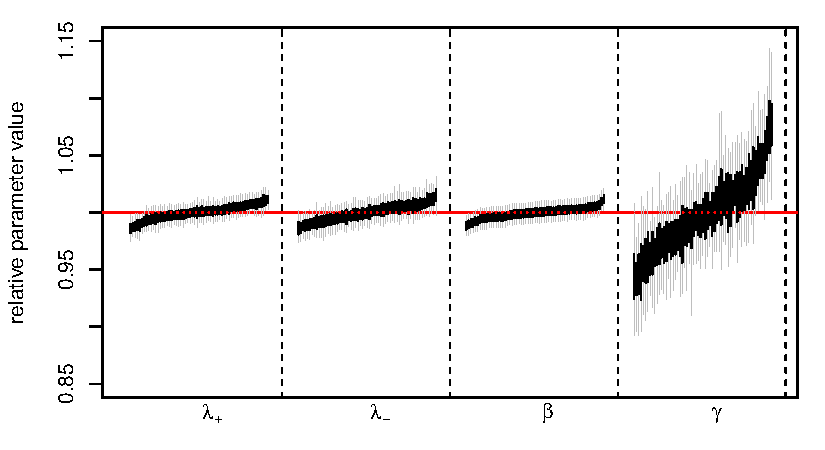
\includegraphics{writeup-plots/coverage_results}
    \end{center}
    \caption{
        Credible intervals for the four parameters of the dynamic Ising model,
        calculated using $(6,2,2)$ T-mers,
        from 61 MCMC runs on independently simulated sequences of $10^6$ bases
        differing at around 18.6\% of the sites.
        Shown are relative intervals, obtained by dividing by the true value.
        \label{fig:ising_coverage}}
\end{figure}


%%%%%%%%%%%
\subsection{Hominid mutation spectrum}

We also applied the method to changes between the human and chimpanzee reference sequences.


\begin{figure}
    \begin{center}
        \includegraphics[width=\textwidth]{writeup-plots/biochem_mcmc_posteriors}
    \end{center}
    \caption{
        Estimated average mutation rates
        for the motifs of Table \ref{tab:hominid_model}
        since the common ancestor of humans and chimpanzee.
        Rates are scaled so that the mean time to common ancestor is 0.001 units --
        if we take this to be 6 million years \citep{scally2012insights,langergraber2012generation}
        then rates are in units of mutations per 6,000 years.
        Shown are posterior medians (points) and 95\% credible intervals (lines, which are quite small in all cases).
        Figure \ref{sfig:biochem_results_zoom} shows the smaller rates in more detail,
        and figure \ref{sfig:biochem_results_relative} shows the rates between categories relative to each other.
        \label{fig:biochem_results}}
\end{figure}

It may seem tenous to look for mutational signatures associated with cancer in the germline,
or absurd that UV damage could play a significant role.
This is in part due to the ``streetlight effect'' --
we can't look for signatures that are not characterized --
but it is also reasonable that shared repair machinery might induce similar context-dependent errors.
More likely sources of error in the germline include the effects of recombination
\citep{arbeithuber2015crossovers,myers2010drive}.

%%%%%%%%%%%%%%%%%%%%
\section{Discussion}

This paper presents a tractable, provably correct method
for doing statistical inference using observations of a particle model
in which probabilities of change are determined only by nearby sites.
Such models appear in many fields, for instance,
as the dynamic counterparts to Markov random fields;
many spin glass models;
and models of DNA sequence evolution.

The methods described here provide a way to efficiently calculate full likelihoods,
which in many circumstances provide the optimal basis for inference \citep{neyman1933problem},
fast enough to allow Bayesian inference from Monte Carlo sampling.
The method is fast thanks to its dependence only only local neighborhoods
(so the time does not scale with sequence length once T-mer abundances are counted)
and its reliance on sparse matrices whose structure can be precomputed and cached.
It avoids approximations made by previous methods thanks to the use of T-mers
and explict quantification of the necessary length of the ``arms'' of the T-mers.
We first discuss possible uses of the method,
followed by challenges (and possible solutions).

\paragraph{Other applications}
One class of applications stems from \emph{inference of process} --
where the numerical values of various mutation rates are directly of interest.
For instance, CpG hypermutability depends on the \nC\nG pair being methylated,
an epigenetic modification that has important consequences for gene regulation;
therefore, inference of CpG mutation rates in ancient taxa provides an indirect estimate
of methylation status in extinct organisms.
Similarly, many mutational motifs are thought to be caused by particular enzymes;
inference of relative rates of these motifs
may provide clues as to the activity and evolution of those enzymes.
Furthermore, iterative model building by examining residual motif counts
could provide a powerful way to discover unknown processes
whose action had been obscured by other sources of noise.

In other applications, reconstruction of an unknown sequence may of interest.
For instance, training data might be used to estimate parameters of a noisy transmission line,
facilitating the later reconstruction of noisily transmitted signals.
Alternatively, multiple observations of independently transmitted copies of a single sequence
(e.g., down a phylogenetic tree)
might be used to estimate the process, and from this infer the original (ancestral) sequence
(or sample from its posterior distribution).

\paragraph{Limitations}
The model presented assumes that the same process occurs at every location along the sequence,
and that the length of the sequnce does not change (no indels).
Neither of these assumptions are likely to be true for any data set of DNA sequence;
however, both assumptions are also made the state of the art in phylogenetics.
Some relaxation of the assumptions is possible -- for instnace,
we can easily allow heterogeneity between sites by scaling rates by an overall gamma-distributed random factor \citep{yang1994maximum}.
Short deletions might be accomodated by introducing a ``gap'' letter to the alphabet,
but insertions may be problematic.


\paragraph{Computation}
The main factor that determines computation time
is the lengths of the T-mers used for inference,
since all computations scale with the number of possible patterns at the long end of the T-mer.
Although the model is efficent enough to deal with fairly long T-mers,
this exponential growth puts hard constraints on the application of the method.
The length of T-mers required to accurately compute the likelihood in most models grows at most linearly
with the mean density of substitution between the initial and final sequence.
This does not in practice greatly increase the length of required T-mer
since substitution densities approaching 100\% are unlikely to be usable in practice
especially if how the sequences align with each other is unknown.
A more serious determining factor of T-mer length is the degree of dependency in the model itself.
For instance, inserting the 13-base pair motif selected against by meiotic drive in primates \citep{myers2010drive}
would require T-mers of width at least 25, and hence vectors of length $4^{25} \approx 1.13 \times 10^{15}$.


\paragraph{Modeling}
Careful building of complex models in this framework may take care,
but no more than in any other class of models (e.g., multivariate linear regression).
It is easy to specify nonidentifiable models --
for instance, all 2mer mutation motifs include the 1mer motifs.
The large number of possible mutation motifs also makes multiple testing an issue;
an unguided approach might include all possible motifs but place a shrinkage prior on their values \citep{bhadra2015horseshoe}.
The converse approach of adding motifs that are overrepresented in the residuals
may be quicker, but entails some degree of arbitrariness in choosing the motifs to add (and in which order).
Finally, inference on trees may be difficult unless the root placement and distribution are strongly constrained:
otherwise, initial investigations suggest the likelihood surface is often strongly ridged --
for instance, increasing the abundance of \nG\ nucleotides at the root while also increasing the mutation rate away from \nG\
can achieve roughly the same result.
However, in phylogenetic applications outgroups can be used to constrain these quantities.

In the genomic context,
if we knew the specific mutational spectrum of each possible repair or copying pathways,
then this framework could be used to rigorously estimate their average usages and impacts.
Despite substantial progress over the past two decades \citep{goodman2013translesion,sale2012yfamily},
this is still far from known.
A promising alternative would be to use the distinct signatures obtained by dimension reduction techniques as in
\citet{alexandrov2013signatures}, \citep{mathieson2017differences} or \citep{shiraishi2015simple} as a proxy for unknown but distinct pathways.

More things to do: cancer; include gaps; more taxa; leading/lagging strand...


\subsection{Acknowledgements}
The initial impetus for this project came from Matt Dean;
along the way substantial encouragement and useful suggestions were provided by
Simon Tavar\'e, Rasmus Nielsen, Graham Coop, Yaniv Brandvain, and Sergey Nuzhdin.
Many thanks are also due Jessica Crisci for curating the human-chimp data.

\bibliography{context-dependence}

\appendix

\section{Supplementary figures}

\begin{figure}
    \begin{center}
        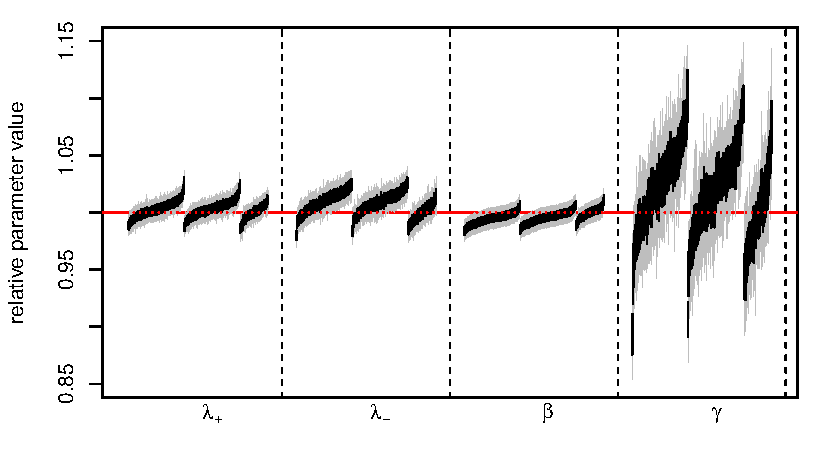
\includegraphics{writeup-plots/coverage_results_all}
    \end{center}
    \caption{
        As in \ref{fig:ising_coverage}:
        Credible intervals for the four parameters of the dynamic Ising model,
        from MCMC runs on independently simulated sequences of $10^6$ bases
        differing at around 18.6\% of the sites.
        Shown are relative intervals, obtained by dividing by the true value.
        The three groups are left to right, credible intervals obtained from $(4,2,1)$, $(5,3,1)$, and $(6,2,2)$ T-mers:
        note that only the longest $(6,2,2)$ T-mers provide well-calibrated coverage (Table \ref{tab:ising_coverage})
        and do not show bias.
        \label{fig:all_ising_coverage}}
\end{figure}

\begin{figure}
    \begin{center}
        \includegraphics[width=\textwidth]{writeup-plots/biochem_mcmc_posteriors_zoomed}
    \end{center}
    \caption{
        As in Figure \ref{fig:biochem_results}, but with reduce vertical axis range
        to see in more detail:
        estimated average mutation rates
        for the motifs of Table \ref{tab:hominid_model}
        since the common ancestor of humans and chimpanzee.
        Rates are scaled so that the mean time to common ancestor is 0.001 units --
        if we take this to be 6 million years \citep{scally2012insights}
        then rates are in units of mutations per 6,000 years.
        Shown are posterior medians (points) and 95\% credible intervals (lines, which are quite small in all cases).
        \label{sfig:biochem_results_zoom}}
\end{figure}

\begin{figure}
    \begin{center}
        \includegraphics[width=\textwidth]{writeup-plots/biochem_mcmc_posteriors_relative}
    \end{center}
    \caption{
        As in Figures \ref{fig:biochem_results} and \ref{sfig:biochem_results_zoom},
        but where each rate is divided by the mean rate across all eight categories
        (as well as the 95\% credible interval endpoints).
        \label{sfig:biochem_results_relative}}
\end{figure}


%%%%
\section{Proof of the approximation}
\label{ss:approx_pf}

First we quantify and prove the approximation \eqref{eqn:window_approx}.
The basic idea is that the probability is only in error if there is a chain of mutations
that create a dependency between the base of the T-mer and the flanking sequence.
To simplify the argument, first assume that all transition triples
change only a single, central site in the pattern,
taking into account context on each side of maximum length $w$.
(For instance, a trinucleotide model in which the flanking sites on each side
affect the mutation rate of the central site has $w=1$.)
%EM I suggest that we could re-introduce the mu^* notation again and remind people that these potential changes are uniform.
Recall that in our construction of the process we first chose the times and sites
at which potential changes might occur.
Suppose a potential change occurs at site $i-w$, at time $t$,
which therefore might result in a change in state at site $i$.
To resolve this, we need to know the outcome of any other potential changes
that might change the sequence between $i-w$ and $i + w$.
Consider those that might happen only to the right of $i$,
thus extending the sequence on which the change depends to the right.
The number of such potential changes is Poisson with mean $\mu^* w t$,
%EM Suggest "and their location is uniform..."
and will extend the amount of sequence on which the change at site $i$ depends
by a uniform random number of sites between 1 and $w$.
If one occurs, say at time $0 < s < t$,
then any further potential changes that occur between time 0 and time $s$
in the $w$ sites to the right of this older potential change
will again extend the range of dependency.
Putting this together, the amount of sequence to the right of a site
on which a mutation at that site depends
is bounded by the compound Poisson process $\sum_{k=1}^N W_k$,
where $N$ is Poisson with mean $\mu^* w t$
and each $W_k$ is independent and uniform on $\{1, 2, \ldots, w\}$.

Now consider the probability of interest,
\begin{align*}
    \P\{ X_{i+\ell}^{(n-\ell-r)}(t) = y \mid X_i^{(n)}(0) = x \} .
\end{align*}
This probability can be written as a sum over all possible arrangements
and resolutions of potential changes.
Our approximation, $p_{n,\ell,r}(x,y)$ is the probability that would be obtained
by ignoring any potential changes that rely on context outside of the $n$-sequence $x$.
So, if $A$ is the event that the final subsequence $y$
depends on sequence outside of $x$ due to potential changes,
then
\begin{align*}
    \left|
        \P\{ X_{i+\ell}^{(n-\ell-r)}(t) = y \mid X_i^{(n)}(0) = x \}
        -
        p_{n,\ell,r}(x,y)
    \right|
    \le \P\{A\} .
\end{align*}
Since the size of the dependency window is a compound Poisson process,
we can bound $\P\{A\}$ using the following lemma:

\begin{lemma}
    Let $X = \sum_{j=1}^N W_j$,
    where $N$ is Poisson with mean $\lambda$
    and each $W_j$ is independent and bounded between 0 and $w$.
    Then for $k \ge 1$,
    \begin{align}
        \P\{ X > k w \}
        \le
        \frac{\lambda^{k+1}}{(k+1)!} .
    \end{align}
\end{lemma}

% # what's this bound look like and how's it compare to a Chebyshev bound
% # that uses the variance of W
%
% ub1 <- function (w, lam, ell=1:10) {
%   k1 <- ceiling(ell/w)
%   return( lam^(k1+1) / factorial(k1+1) )
% }
% # the Chebyshev bound never does better
% ub2 <- function (w, lam, ell=1:10) {
%   k2 <- (ell - lam * (w+1) / 2) / w
%   return( lam * (w+1) * (2*w+1) / (6 * w^2 * k2^2) )
% }
% wvals <- c(1, 2, 3)
% ub1mat <- sapply(wvals, ub1, lam=0.75)
% ub2mat <- sapply(wvals, ub2, lam=0.75)
% matplot(ub1mat, type='l', lty=1)
% matlines(ub2mat, type='l', lty=2)
% legend('topright', lty=1, col=seq_along(wvals), legend=sprintf("w=%d", wvals))

\begin{proof}
    First note that $\P\{X > kw\} \le \P\{N > k\}$.
    Now, use the fact that if $f(n) = n (n-1) \cdots (n-k) / (k+1)!$
    then $f(n) = 0$ for integers $0 \le n \le k$ and $f(n) \ge 1$ for $n > k$,
    and so $\P\{N > k\} \le \E[f(N)]$.
    Now, $\E[f(N)] = \lambda^{k+1} / (k+1)!$ via direct calculation or the
    formula for the $k+1$st factorial moment for the Poisson distribution.
\end{proof}

Putting this together,
we find that
\begin{align*}
    \left|
        \P\{ X_{i+\ell}^{(n-\ell-r)}(t) = y \mid X_i^{(n)}(0) = x \}
        -
        p_{n,\ell,r}(x,y)
    \right|
    \le
    \frac{
        2 (\mu^* t)^{k+1}
    }{
        (k+1)!
    } .
\end{align*}
Here, the factor of 2 comes from the two sides (to the left and right) of the base of the T-mer.

The argument applies to more general transition triples,
with $w$ set equal to the maximum distance
from a position that is changed to the edge of the context
across all transition triples.


\paragraph{Full likelihood}
Now we use these ideas to quantify and prove approximation~\eqref{eqn:full_approx}.
For two positions $(i,s)$ and $(j,t)$ in sequence $\times$ time,
let $r(i,s;j,t) = |j-i|/|t-s|$ be the slope of the line between them,
and if $I$ and $J$ are subsets of sites, let $r(I,s;J,t) = \min\{r(i,s;j,t) : i\in I, j \in J\}$
be the minimum.
Above we have shown that there is a speed of dependency propagation $r_*$
such that if $r(I,s;J,t) > r_*$,
then $X_I(s)$ and $X_J(t)$ are nearly independent.
Now, fix $t$ and for each site $i$ let $N_i$ denote its $r_*$-neighborhood,
i.e.,
\begin{align}
%EM Before we had i,s,j,t, and now we have i,t,j,s. It doesn't make a difference, but should we choose one?
%EM Do we want to specify a max allowable range for j as well on the RHS?
    N_i = \{ (j,s) : r(i,t; j,s) \le r_*, \; 0 \le s \le t \} .
\end{align}
These are depicted in Figure~\ref{fig:neighborhoods}A.
We will write $i \sim j$ if $|i-j| \le 2 r_* t$,
or equivalently, if $N_i \cap N_j \neq \emptyset$,
and $i \nsim j$ otherwise.
We can think of $N_i$ as the parts of ancestral sequences in which a mutation might have affected the state at $(i,t)$,.
so if $i \nsim j$, then $i$ and $j$ are (approximately) independent at time $t$, given the sequence at time 0.
Concretely,
we have a small $\epsilon$ such that for any $i \nsim j$,
\begin{align*}
    &\big|
    \log( \P\{ X_i(t) = x_i \text{ and } X_j(t) = x_j \} ) \\
    &\qquad {} -
    \log( \P\{ X_i(t) = x_i \} \P\{ X_j(t) = x_j \} )
    ) \big|
    \le \epsilon .
\end{align*}


\begin{figure}
    \begin{center}
    %EM This looks like N12 to me. Am I miscounting?
    %EM I suggest we include t and s in the diagram too.
        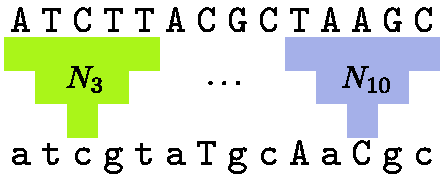
\includegraphics{context-neighborhoods-defns}

        \vspace{2em}

        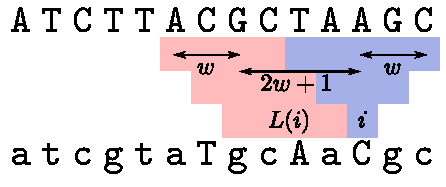
\includegraphics{context-neighborhoods-widths}
    \end{center}
    \caption{
        %EM TODO make this A and B so we can refer to them in the text.
        Diagram of things in the text:
        (top) Dependency neighboorhods.
        (bottom) What we need to compute $\P\{X_i(t)=x \given X(0), X_{<i}(t)\}$:
        site $i$ depends on the blue squares in $N_i$;
        the sites to the left of this in $L(i)$ are those other sites in $X(t)$
        whose dependency neighborhoods overlap $N_i$;
        any further sites to the left of this are basically independent of $X_i(t)$;
        the red squares give the dependency neighborhood of $L(i)$,
        so we need to condition on the row of red and blue sites at the top.
        On the bottom, we have $2w+1$ sites; at the top we have $4w+1$;
        here $w=2$.
        \label{fig:neighborhoods}
    }
\end{figure}


What we'd like to know is the likelihood, i.e.,
\begin{align}
    \like(y|x)
    &:=
    \P\{ X(t) = y \given X(0) = x \} .
\end{align}
If we define $X_{<i}=(X_1, \ldots, X_{i-1})$, then
\begin{align}
    \like(y|x)
    &=
    \prod_{i=1}^n
    \P\{ X_i(t) = y_i \given X(0) = x \text{ and } X_{<i}(t) = y_{<i} \} .
\end{align}
Now, defining $L(i) = \{ j < i \st j \sim i \}$
to be the sites to the left of $i$ whose dependency neighborhoods overlap with $i$'s,
and $A(I) = \{ j \st |j-i| \le r_*t \text{ for some } i \in I\}$
to be the ancestral sites in the dependency neighborhood of $I$,
\begin{align}
&\big|
    \log( \P\{ X_i(t) = y_i \given X(0) = x \text{ and } X_{<i}(t) = y_{<i} \} ) \\
& \qquad {} -
    \log( \P\{ X_i(t) = y_i \given X_{A(L(i))}(0) = x_{A(L(i))} \text{ and } X_{L(i)}(t) = y_{L(i)} \} )
 \big| \\
&\qquad \qquad \le
    \epsilon ,
\end{align}
so that if we define
\begin{align}
    \alike(y|x)
    &=
    \prod_{i=1}^n
    \P\{ X_i(t) = y_i \given X_{A(L(i))}(0) = x_{A(L(i))} \text{ and } X_{L(i)}(t) = y_{L(i)} \} ,
\end{align}
then (with $\loglike = \log \like$),
\begin{align}
    \left| \aloglike(y|x) - \loglike(y|x) \right|
    \le n \epsilon .
\end{align}

This is good, because we can compute $\aloglike$:
let $w=r_*t$ be radius of a dependency neighborhood,
so that the width of $L(i)$ is $2w$,
and for a sequence $x$ define $x^{(m)}_i = (x_{i-m+1}, \ldots, x_i)$:
\begin{align}
    \alike(y|x)
    &=
    \prod_{i=1}^n
    \frac{
        p_{w,2w+1}(y^{(2w+1)}_i|x^{(4w+1)}_{i+w})
    }{
        p_{w,2w}(y^{(2w)}_{i-1}|x^{(4w)}_{i-1+w})
    }
\end{align}
This is the ratio of the likelihoods of all the $(w,2w+1)$ T-mers,
divided by the likelihoods of all the $(w,2w)$ T-mers.




\section{Peeling algorithm}
\label{ss:peeling_algorithm}

Fix one tip of the tree, $a$, to be the taxa where we count ``long'' sequences, let $\rho$ be the root, and let $b_1, \ldots, b_n$ be the remaining tips,
where we observe ``short'' sequences.
Let $v_0=\rho, v_1, \ldots, v_\ell = a$ be the path from the root down to $a$,
let $u_1, u_2, \ldots, u_m$ be the remaining internal nodes,
and for each $v_i$ let $u(v_i)$ be the offspring of $v_i$ that is not one of the other $v$.
For each node in the tree,
we will compute a matrix of probabilities:
for nodes not on the path from $a$ to the root,
we compute the chance that that each ``long'' sequence observed at that node
is matched by each possible combination of ``short'' sequences on the tips of the tree below it.
For nodes on the path from $a$ to the root, we compute the probability of observing
each ``long'' sequence at that node, along with the combinations of ``short'' sequences
on all tips further away from $a$ (i.e., below that node if it was rooted at $a$).
For a node $w$ this will be stored as a $|\calS|^{n} \times |\calS|^{cm}$ matrix, for some $c$,
and denoted $M(w)$.
Rows of $M(u_j)$ sum to 1,
while each entire matrix $M(v_i)$ sums to 1;
the difference being that $M(v_i)$ sums over the prior at the root,
and $M(u_j)$ takes the value at $u_j$ as given.

Let $t(w)$ be the length of the branch above node $w$, for $w \neq \rho$,
and denote by $G^T$ the transpose of $G$.

\begin{enumerate}

  \item Set $M(b_i) = P$ for each $b_i$.

  \item While there are $u_j$ whose children $w_1$ and $w_2$ both have matrices computed,
    \begin{enumerate}
      \item let
        \begin{align}
          M(u_j)_{x,(y,z)} = \left( e^{t(w_1) G} M(w_1) \right)_{x,y} \left( e^{t(w_2) G} M(w_2)_{x,z} \right)_{x,z} .
        \end{align}
    \end{enumerate}

  \item Let
    \begin{align}
      M(\rho)_{x,y} = \pi(x) \left( e^{t(u(\rho)) G} M(w(\rho)) \right)_{x,y}
    \end{align}

  \item For each $1 \le k < \ell$,
    \begin{enumerate}
      \item let
        \begin{align}
          M(v_k)_{x,(y,z)} = \left( e^{t(v_k) G^T} M(v_{k-1}) \right)_{y,x} \left( e^{t(u(v_k)) G} M(u(v_{k-1})) \right)_{x,z}  .
        \end{align}
    \end{enumerate}

  \item Finally, let
    \begin{align}
      M(a)_{x,y} = \left( e^{t(a) G^T} M(v_{\ell-1}) \right)_{x,y}  .
    \end{align}

\end{enumerate}


%%%%
\section{Other likelihood functions}

\subsection{Summary statistics}

Since we cannot compute reasonably the full likelihood for the data,
we will need to choose appropriate summary statistics
that contain as much information about the process as possible,
and have a tractable expression for their marginal likelihood.
For simplicity,
we assume in this section that approximation \eqref{eqn:window_approx} holds exactly.
If $i_1 < \ldots < i_{n(x)}$ are a set of nonoverlapping sites where the initial sequence matches $x$
-- i.e., $X_{i_k}^{(2\ell+m)}(0)=x$ and $i_{k+1} > i_k + 2\ell+m$ for all $k$ %En dash close to math could be confusing. This sentence is a doozy.
then the counts $N(x,y)=\#\{ i_k \st X_{i_k+\ell}^{(m)}(t)=y\}$ (the number of these sites that match the smaller pattern $y$ at time $t$)
are multinomial, with probabilities $\{p_{\ell,m}(x,y)\st y \in \calS^m\}$.
For instance, if $\ell=3$ then $N(\text{ACTCAC}, \text{CGC})$ counts the number of occurrences of
\begin{center}
\begin{tabular}{c|ccccccc}
 $x$ &  C  & A & C & T & C & A & C \\
 $y$ &  $\centerdot$  & $\centerdot$  & C & G & C & $\centerdot$  & $\centerdot$
\end{tabular}
\end{center}
where $\cdot$ represents any base.
More generally, if we partition the sequence into windows of length $2\ell+m$,
and let $N(x,y)$ be the number of times we see a window in which $x$ matches $X(0)$ and $y$ matches $X(t)$,
then these counts are independently multinomial across each $x$.
% so the marginal likelihood of the statistics $N(x,y)$ is
% \begin{align}
%     \prod_{x \in \calS^{2\ell+m}} N(x)! \prod_{y \in \calS^m} \frac{p_{\ell,m}(x,y)^{N(x,y)}}{N(x,y)!} ,
% \end{align}
% where $N(x) = \sum_y N(x,y)$.

Of course, a drawback to this approach is that we throw away a good fraction of the data.
In fact, we do not even look at a fraction $2\ell/(2\ell+m)$ of the second sequence, $X(t)$,
that lies in the outside edges of each window.
As before, let $N(x)$ be the number of occurrences of a pattern $x$ in $X(0)$,
and $N(x,y)$ the number of times $x$ is seen juxtaposed with $y$ in $X(t)$,
but this time, count over all positions,
so that e.g., $N(x) = \#\{ 1 \le i \le n - 2\ell - m + 1 \st X_i^{(m+2\ell)}(0)=x\}$.

Now we will now calculate the expectation and covariances of $N(x,y)$.
\peter{The following is Not Right, but also we don't really use it at the moment.}
If we assume that \eqref{eqn:window_approx} is exact, then
\[
    \E [N(x,y)] = N(x) \, p_{\ell,m}(x,y).
\]
To compute covariances, define $\chi_i(x,y)$ to be 1 if $X_{i-\ell}^{(|x|)}(0)=x$ and $X_i^{(|y|)}(t)=y$, and 0 otherwise,
so that $N(x,y) = \sum_{i=1}^n \chi_i(x,y)$.
Overloading notation, also define $\chi_i(x)$ to be 1 if $X_{i-\ell}^{(|x|)}(0)=x$,
\begin{align}
  \var[N(x,y)] &= \sum_{i=1}^n \var[\chi_i(x,y)] + \sum_{i\neq j} \cov[\chi_i(x,y), \chi_j(x,y)] \\
               &\approx \sum_{i=1}^n \chi_i(x) p_{\ell,m}(x,y)(1-p_{\ell,m}(x,y))
            + 2 \sum_{i=1}^{n-2\ell-m} \sum_{j=i+1}^{i+2\ell+m-1} \cov[ \chi_i(x,y) \chi_j(x,y) ] \\
            &= N(x) p_{\ell,m}(x,y)(1-p_{\ell,m}(x,y)) +
\end{align}
The term $\E[\chi_1(x,y) \chi_{k+1}(x,y)]$ is the probability that $x$ matches at both site 1 and site $k+1$,
and that $y$ matches both at site $\ell+1$ and at site $\ell+k+1$.
For this to be nonzero, the joint pattern $(x,y)$ must allow self-overlaps.
Similarly, if $(x_1,y_1) \neq (x_2,y_2)$ then
\begin{align}
  \begin{split}
    \cov[N(x_1,y_1),N(x_2,y_2)]
    & \approx - n (2m+4\ell) p_{\ell,m}(x_1,y_1)p_{\ell,m}(x_2,y_2) \\
    & \qquad {} + n\sum_{k=1}^{m+2\ell} \E[\chi_1(x_1,y_1) \chi_{k+1}(x_2,y_2) + \chi_1(x_2,y_2) \chi_{k+1}(x_1,y_1)] .
  \end{split}
\end{align}


%%%%
\subsection{A likelihood function}

The covariance calculations show that
if $p_{\ell,m}(x,y)$ is small enough (i.e., the pattern is not common),
then $N(x,y)$ is close to Poisson.
Using this observation, we can estimate parameters by composite likelihood,
using all $N(x,y)$ as data.
Specifically, this composite likelihood is
\begin{align} \label{eqn:comp_like}
  \prod_{x,y} F_{(x,y)}^{N(x,y)}
\end{align}
where $F$ is the $|\calS|^{m+2\ell} \times |\calS|^m$ matrix whose $(x,y)^\text{th}$ entry is $p_{m,\ell}(t,x,y)$ as described in the "Computation" section.
Maximum likelihood then gets an asymptotically unbiased estimate of the parameters. (cite)
However, since they are not independent, to get confidence intervals, we need to either simulate, or do something different.

If we use only a subset of patterns $\{(x_k,y_k)\}$ chosen so that $\E[M_1(x,y) M_{k+1}(x,y)]$ is small (or zero),
\erick{M not defined, but I'm guessing that this is effectively saying that the probability of having two different patterns apply to the same sequences is small?}
the entire collection $\{N(x_k,y_k)\}$ will be close to independent Poisson.
(using Stein's method)
Then we'll have the correct likelihood function for (this subset of) data.

If changes are rare, then one way to get a set of patterns with this property is to only choose ones such that going from $x$ to $y$ entails a change;
and any overlapping patterns must require additional changes,
i.e., if $(x_1,y_1)$ matches at $i_1$,
then for $(x_2,y_2)$ to match at $i_2$,
there must be additional changes outside $(i_1,\ldots,i_1+\ell-1)$.

Here is one way to obtain such a set.
Take a pair of patterns $(x,y)$, that overlap at $m$ positions,
and suppose that they differ at $1 \le i_1, \ldots, i_d \le m$.
Let $\bar i = (1/d) \sum_{j=1}^d i_j$ be the mean position of the changes,
and take only patterns with $(m-1)/2 < \bar i \le (m+1)/2$.
For example, in the example above with $m=3$ and $\ell=2$,
\begin{center}
\begin{tabular}{c|ccccccc}
 $x$ &  C  & A & C & T & C & A & C \\
 $y$ &  $\centerdot$  & $\centerdot$  & C & G & C & $\centerdot$  & $\centerdot$
\end{tabular}
\end{center}
$x$ and $y$ differ only at (relative) position $i_1=2$.

Another way to achieve the same goal of having all overlapping patterns require additional changes is to require $i_1 = \bar i = 1$.
No two such patterns can be shifted versions of each other
without adding more changed sites,
since shifting by $k$ without adding changed sites just adds $k$ to $\bar i$.
For example, we might take
\begin{center}
\begin{tabular}{c|ccccccc}
 $x$ &  A & C & T & C & A & C & G \\
 $y$ &  $\centerdot$  & $\centerdot$  & G & C & A & $\centerdot$  & $\centerdot$
\end{tabular}
\end{center}

\section{Removed bits that we probably don't want}

\subsection{s5f likelihood}

The s5f model is defined as follows:
for each $(a,b,c,d,e,x) \subset \{\nA,\nC,\nG,\nT\}$,
it gives a (relative) mutation rate
\begin{align}
    \gamma(c,x;a,b,d,e) = \text{( mutation rate of $c \to x$ in context $abcde$ )} .
\end{align}
Given these rates, the only unknown parameter is the total amount of time
that the sequence has been mutated for.
Suppose that $X(t)$ is a sequence of length $n$ evolving under this model,
and let $G_n$ be the corresponding generator matrix,
a $4^n \times 4^n$ matrix.
(In the s5f model, the mutation rates are only specified in the middle of 5-mers,
so the two bases on each end never mutate.)
The transition probabilities are $e^{tG_n}$,
and by marginalization,
we can compute quantities like
the probability for observing the middle set of basis
given the flanking $\ell$ on each end:
\begin{align}
    p_{\ell,n-2\ell}(t;a,b)
    &=
    \P\{
        (X_{\ell+1}(t), X_{\ell+2}(t), \ldots, X_{n-\ell}(t))=(b_1,b_2,\ldots,b_{n-2\ell}) \\
    &\qquad \qquad
        \given (X_{1}(0), X_{2}(0), \ldots, X_{n}(0))=(a_1,a_2,\ldots,a_{n})
    \} .
\end{align}
If the size of the context, $\ell$, is big enough,
then this probability will not depend significantly if the sequence $a$ is in fact embedded in a longer sequence
(the error decreases exponentially with $\ell$).

The sequence $X(t)$ can be constructed by beginning with $X(0)$,
putting down a Poisson process of potential mutations of rate $\gamma = \max\{\gamma(c,x;a,b,d,e)\}$,
and thinning appropriately.
The process depends on the flanking 2bp,
so any other mutation within 2bp of a site affects the process at that site,
and the chance that this occurs depends on the flanking 4bp on either side.
Concretely, the number of flanking positions in each direction
that must be kept track of to decide what happens at a given site
grows by 1 at rate $\gamma$, and by 2 at rate $\gamma$;
so the amount of flanking sequence on each side affecting a given site at time $t$
is the sum of a Poisson($\gamma t$) and twice an independent Poisson($\gamma t$).
This has mean $3\gamma t$ and variance $5 \gamma t$;
with high probability it will not exceed, say,
$3\gamma t + 6 \sqrt{\gamma t}$;
if $\gamma t < 1$ this is less than 9.



%%%%%%%%
\subsection{Edge effects and cyclicization}

The choice to treat long sequences as cyclical is generally of little importance.
However, we have defined in \eqref{eqn:G_defn} the basic building block of our approximation, $G(m)$,
to be the transition matrix \emph{for a circular sequence} of length $m$, where $m$ may be short.
\peter{no we haven't}
This seems strange -- but, what else would we do at the edges?
We want to use $G(\ell+m+r)$ to compute the chance that a given $(\ell+m+r)$-sequence ends up with another given $m$-sequence in the middle;
and if $\ell$ and $r$ are big enough relative to $t$, this will be a good approximation regardless of what we do at the edges.
One answer would be to not allow patterns hanging off of either end to match,
resulting in a slight underestimate of the chance of change.
A better approximation would be to use the marginal frequencies in some way to average over surroudning sequence
-- but, this requires marginal frequencies to be known, and these are not stationary.
However, the leftmost site in a randomly chosen window is a sample from the marginal distribution,
and if sites separated by distance $\ell+m+r$ are sufficiently uncorrelated,
wrapping the sequence around is a good approximation to averaging over marginal frequencies in the surrounding sequence.
It is easy to imagine situations where this would not be the best solution --
but again, if $\ell$ and $r$ are large enough, it won't matter much.

%%%%
\subsection{The root distribution}

We clearly don't want to add an extra parameter $\pi(z)$ for all $z \in \calS^{m+2\ell}$.
If nothing else, it would make the inference depend on $m$ and $\ell$, which we'd like to avoid.
One approach would be to put a Dirichlet distribution on $\pi(z)$.
This has the nice property that you can choose priors that are consistent across different values of $m$ and $\ell$.
We'd have to still MCMC around in the space of $\pi(z)$, so they'd be nuisance parameters from that point of view.
Also, making the frequencies at the root random introduces correlations between counts, which we want to avoid.
An alternative is to specify $\pi$ through lower-dimensional statistics,
for instance to model the root state as a sample from a Markov random field
with parameters for the marginal frequencies of each state, and pairwise (or higher) correlations between them.

A Markov random field with interactions between sites no more than distance two away
is determined by the energy function $\phi(a,b,c)$ which gives the ``energy'' of the configuration $abc$ for each $a,b,c \in \calS$.
We use this to define the distribution on root patterns $\pi$ by
\begin{align}  \label{eqn:root_mrf}
    \pi(z) = \frac{1}{Z} \exp\left( - \sum_{i=1}^{|z|} \phi(z_{i-1},z_i,z_{i+1}) \right),
\end{align}
i.e., the exponential of the total energy of each three adjacent sites,
where $Z$ is the normalizing constant.
Note that it is often difficult to compute $Z$ in applications of Markov random fields,
but here we are working with relatively short sequences,
so we just compute \eqref{eqn:root_mrf} for all possible $z$, and divide by the sum.
(However, for this same reason this is not equivalent to saying that $X(0)$ is a sample from the Markov random field
and finding the distribution of patterns within this.)


%%%%%
\subsubsection{Mixing}

There can be significant confounding of the frequencies at the root with the other parameters,
which results in poor mixing.
(See CpG results, below.)
To see why this is, consider the following back-of-the-envelope calculation.
Take $x \neq y$ to be single bases (so, set $\ell=0$ and $w=1$),
so that $N(x,y)$ gives the number of times an $x$ and a $y$ are homologous.
Let $q(x,y)$ be the instantaneous rate that $x \to y$ (averaged somehow over context?),
so that $N(x,y)$ should be, roughly,
\begin{align*}
  \sum_z \pi(z) q(z,x) q(z,y) &\approx t \pi(x) (1+q(x,x)) q(x,y) + t \pi(y) q(y,x) (1+q(y,y)) ,
\end{align*}
where as usual $q(x,x) = (-1) \sum_{z \neq x} q(x,z)$ is (minus) the total jump rate out of $x$.

So, when we propose a change to $\pi$ we might want to also adjust the rates accordingly to keep this more-or-less constant:
if we chnage $\pi(x) \mapsto \pi(x) + \epsilon_x$, we want $\delta_{xy}$ to satisfy
\begin{align*}
  \sum_z \pi(z) q(z,x) q(z,y) = \sum_z (\pi(z) + \epsilon_z) ( q(z,x) + \delta_{zx} ) ( q(z,y) + \delta_{zy} ) ,
\end{align*}
or, to first order in $\delta$,
\begin{align*}
  0 &\approx \sum_z \epsilon_z q(z,x) q(z,y) + \sum_z \pi(z) \delta_{zx} q(z,y) + \sum_z \pi(z) q(z,x) \delta_{zy} \\
   &\approx \sum_z \epsilon_z q(z,x) q(z,y) + \sum_z (\pi(z)+\epsilon_z) \delta_{zx} q(z,y) + \sum_z (\pi(z)+\epsilon_z) q(z,x) \delta_{zy} \\
   &\approx \epsilon_x (1+q(x,x)) q(x,y) + \epsilon_y q(y,x) (1+q(y,y)) + (\pi(y)+\epsilon_y) \delta_{yx} (1+q(y,y)) + (\pi(x)+\epsilon_x) (1+q(x,x)) \delta_{xy} \\
   &= \left( \epsilon_x q(x,y) + (\pi(x)+\epsilon_x) \delta_{xy} \right)(1+q(x,x)) + \left( \epsilon_y q(y,x) + (\pi(y)+\epsilon_y) \delta_{yx} \right)(1+q(y,y))
\end{align*}
One solution to this is to let $\delta_{xy} = - \epsilon_x q(x,y) / \pi(x)$.

Suppose each change is a single-base change, so that changes $\delta \mu_i$ in $\mu$ contribute to $q$ by
$\delta_{xy} = \sum_{i: x \to y} \delta \mu_i$.
Given $\delta_{xy}$, this gives a linear equation for $\delta \mu_i$ that may or may not be solvable,
but certainly is if we have all the single-base transitions as paramters.

\subsection{Models without using potential}

Here is a reformulation of the CpG and Ising models without using a potential.

\begin{example}[CpG mutation]
    \peter{version without selection}
  A sequence of genome can be written using A, C, G, and T;
  in the most general model of independent mutation across sites, each of the 12 possible transitions occurs at its own rate.
  Furthermore, it is a well-known observation that in many species,
  adjacent, methylated CG dinucleotides (``CpG sites'') have a much higher mutation rate to TG and CA
  than either single nucleotide change under the independent model.
  Embellishing the single-nucleotide model with this additional rate results in the model defined by

  \begin{center}
    \begin{tabular}{c@{\quad$\to$\quad}c@{\quad at rate\quad }cc}
      $x$  &  $y$  &  $m_{xy}$ & when $x \neq y \in \{\nA,\nC,\nG,\nT\}$  \\
      \nC\nG   &  \nT\nG   &  $\gamma$ & \\
      \nC\nG   &  \nC\nA   &  $\gamma$ &
    \end{tabular} .
  \end{center}
  Here $\gamma$ is the additional CpG rate above the base mutation rate,
  and a total of 13 parameters.
  Note that this model is very different in spirit to TASEP,
  in which the total number of particles was conserved.

  In this model, for a given pair of sequences, there may be more than one way to mutate a given string $x$ to get $y$:
  for instance, a change $\nA\nC\nG \to \nA\nT\nG$ could have occurred by a single $\nC \to \nT$ mutation,
  or by a $\nC\nG \to \nT\nG$ mutation;
  and hence the total instantaneous rate at which ACG changes to ATG is $\gamma + m_{\nC\nT}$.
  Although this means there are many possible parameterizations,
  note that the model is identifiable, not overparameterized.

\end{example}


\begin{example}[1-D Ising model with Glauber dynamics]
    \peter{version without selection}
  In the Ising model, each site is labeled as either ``up'' or ``down'' ($+1$ or $-1$ respectively),
  imagined as magnetic dipoles,
  and the energy associated with a given state $x$ is $H(x) = - \frac{1}{2} \beta \sum_i x_i x_{i+1} - \frac{1}{2} \gamma \sum_i x_i$.
  Here $\beta$ represents inverse temperature, and $\gamma$ represents the strength of the magnetic field (here scaled by temperature).
  The associated stationary distribution on configurations is proportional to $\exp(-H(x))$.
  The following ``Glauber dynamics'' preserve the stationary distribution:
  each site, independently at rate $\lambda$,
  forgets its spin,
  and reconfigures to a state chosen with probability proportional to the stationary probability of the resulting configuration.
  Ignoring transitions that don't change the state,
  if patterns $u$ and $v$ differ at only one site then $u$ changes to $v$ at rate $\lambda/(1+\exp(H(v)-H(u)))$,
  so

    \peter{reformulate with a potential}

  \begin{center}
    \begin{tabular}{c@{\quad$\to$\quad}c@{\quad at rate\quad }c}
      $+++$  &   $+-+$   &  $\lambda/\,(1+e^{2\beta + \gamma})$ \\
      $++-$  &   $+--$   &  $\lambda/(1+e^{\gamma})$ \\
      $+-+$  &   $+++$   &  $\lambda/(1+e^{-2\beta - \gamma})$ \\
      $+--$  &   $++-$   &  $\lambda/(1+e^{-\gamma})$ \\
      $-++$  &   $--+$   &  $\lambda/(1+e^{\gamma})$ \\
      $-+-$  &   $---$   &  $\lambda/(1+e^{-2\beta + \gamma})$ \\
      $--+$  &   $-++$   &  $\lambda/(1+e^{-\gamma})$ \\
      $---$  &   $-+-$   &  $\lambda/(1+e^{2\beta - \gamma})$
    \end{tabular}
  \end{center}


\end{example}


\subsection{Longer models}
      \begin{center}
          \begin{tabular}{c@{\;\;$\to$\;\;}c@{\;\; {\small at rate}\;\; }c|c@{\;\;$\to$\;\;}c@{\;\; {\small at rate}\;\; }c|c@{\;\;$\to$\;\;}c@{\;\; {\small at rate}\;\; }c}
            \nT\nC     &   \nT\nT      &  $\mu_{UV1}$    & \nC\nG       &   \nC\nT       &  $\mu_{g}$       & \nA\nA\nC\nT  &   \nA\nA\nT\nT   &  $\mu_{\AID}$ \\
            \nG\nA     &   \nA\nA      &  $\mu_{UV1}$    & \nC\nG       &   \nA\nG       &  $\mu_{g}$       & \nA\nA\nC\nC  &   \nA\nA\nT\nC   &  $\mu_{\AID}$ \\
            \nC\nC     &   \nC\nT      &  $\mu_{UV2}$    & \nT\nC\nA    &   \nT\nT\nA    &  $\mu_{\APOBEC}$ & \nA\nG\nC\nT  &   \nA\nG\nT\nT   &  $\mu_{\AID}$ \\
            \nG\nG     &   \nA\nG      &  $\mu_{UV2}$    & \nT\nC\nT    &   \nT\nT\nT    &  $\mu_{\APOBEC}$ & \nA\nG\nC\nC  &   \nA\nG\nT\nC   &  $\mu_{\AID}$ \\
            \nC\nC     &   \nT\nT      &  $\mu_{UV3}$    & \nT\nC\nA    &   \nT\nG\nA    &  $\mu_{\APOBEC}$ & \nA\nA\nC\nT  &   \nA\nA\nT\nT   &  $\mu_{\AID}$ \\
            \nG\nG     &   \nA\nA      &  $\mu_{UV3}$    & \nT\nC\nT    &   \nT\nG\nT    &  $\mu_{\APOBEC}$ & \nA\nA\nC\nC  &   \nA\nA\nT\nC   &  $\mu_{\AID}$ \\
            \nT\nC\nG  &   \nT\nT\nG   &  $\mu_{mUV}$    & \nT\nG\nA    &   \nT\nA\nA    &  $\mu_{\APOBEC}$ & \nA\nG\nC\nT  &   \nA\nG\nT\nT   &  $\mu_{\AID}$ \\
            \nC\nC\nG  &   \nC\nT\nG   &  $\mu_{mUV}$    & \nA\nG\nA    &   \nA\nA\nA    &  $\mu_{\APOBEC}$ & \nA\nG\nC\nC  &   \nA\nG\nT\nC   &  $\mu_{\AID}$ \\
            \nC\nG\nA  &   \nC\nA\nA   &  $\mu_{mUV}$    & \nT\nG\nA    &   \nT\nC\nA    &  $\mu_{\APOBEC}$ & \nT\nA\nC\nT  &   \nT\nA\nT\nT   &  $\mu_{\AID}$ \\
            \nC\nG\nG  &   \nC\nA\nG   &  $\mu_{mUV}$    & \nA\nC\nA    &   \nA\nC\nA    &  $\mu_{\APOBEC}$ & \nT\nA\nC\nC  &   \nT\nA\nT\nC   &  $\mu_{\AID}$ \\
            \nT\nA     &   \nT\nG      &  $\mu_{\eta}$   & \nA\nA       &    \nA\nG      &  $\mu_{\iota1}$  & \nT\nG\nC\nT  &   \nT\nG\nT\nT   &  $\mu_{\AID}$ \\
            \nT\nA     &   \nC\nA      &  $\mu_{\eta}$   & \nT\nT       &    \nC\nT      &  $\mu_{\iota1}$  & \nT\nG\nC\nC  &   \nT\nG\nT\nC   &  $\mu_{\AID}$ \\
            \nA\nA     &   \nG\nT      &  $\mu_{\iota2}$ & \nT\nG\nC\nT &  \nT\nG\nT\nT  &  $\mu_{\AID}$    & \nT\nA\nC\nT  &   \nT\nA\nT\nT   &  $\mu_{\AID}$ \\
            \nT\nT     &   \nA\nC      &  $\mu_{\iota2}$ & \nT\nG\nC\nC &  \nT\nG\nT\nC  &  $\mu_{\AID}$    & \nT\nA\nC\nC  &   \nT\nA\nT\nC   &  $\mu_{\AID}$
        \end{tabular}
      \end{center}

\end{document}
